
\section{Introduction}

In traditional datacenters, the practice is to either follow
a dedicated model and provision servers for peak loads, or share
resources in a best-effort manner that offers no
guarantees~\cite{resource-overbooking}.
For example, an auction website may be hosted on a single PM
in order to guarantee that it has enough resources to face peak loads.
However, this
results in under-utilization of resources and wastage of power during
low loads, say, when the auction website is idle during night.
Alternatively, co-hosting the auction website with another service 
in simply a
best-effort manner will be insufficient when either of the
co-hosted services is bombarded with heavy load.
Resource utilization can be maximized while still ensuring performance
guarantees through dynamic resource provisioning~\cite{sandpiper, 
vm-multiplexing}, by adopting virtualization
and consolidating/co-hosting multiple services (like
auction websites and email servers) as VMs on the same physical
machine~\cite{entropy}.

Several to-be-virtualized applications have data dependencies
between each other or among their components.
Example instantiations are, (i)~a multi-tier web-based application has
exchange of data
between its components\textemdash{}web-server, application logic server
and the database, and 
(ii)~heavily parallelized applications~\cite{high-consuming-parallel}
which have distributed computing tasks with mutual data dependencies.
\textit{Server consolidation} refers to mapping a set of applications/servers
to instances hosted within
virtual machines, in such a way as to maximize the utility of the
available infrastructure~\cite{load-balancing}.
Thus, server consolidation can facilitate sharing of available resources
among the tiers of a single application or 
across tiers of multiple applications,
using dynamic resource allocation and virtual machine
migration techniques~\cite{sandpiper, adaptation-engine}.


\begin{figure}[h]
	\centering
	\subfloat[Before Consolidation]{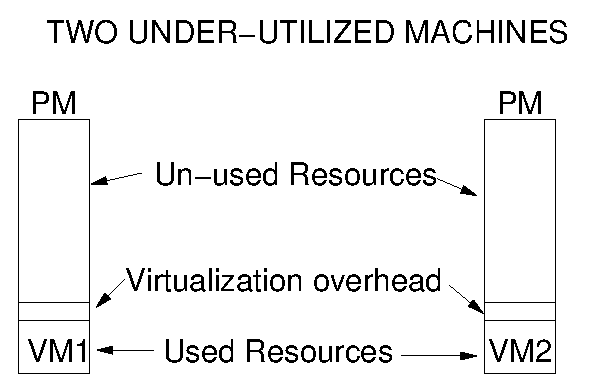
\includegraphics[height=4cm,width=5cm]{figures/before_consolidation.eps}}
	~~~~~~~~~~~~~~~~~~~~~~~~
	\subfloat[After Consolidation]{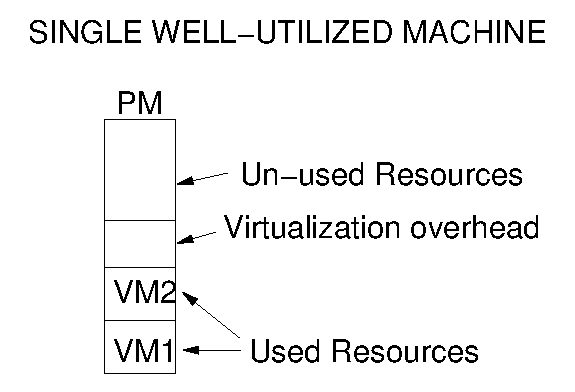
\includegraphics[height=4cm,width=5cm]{figures/after_consolidation.eps}}
\caption{Server Consolidation, via Virtualization, for efficient resource multiplexing.}
\label{virtualization-enables-consolidation}
\end{figure}

An example consolidation scenario is shown in Fig.~\ref{virtualization-enables-consolidation}, 
where two virtualized server instances are moved to or co-hosted on a single physical machine 
such that only one physical machine is sufficient to host both services and
the other machine which becomes idle can be powered off.
In the ``Before Consolidation'' case of Fig.~\ref{virtualization-enables-consolidation}(a), 
each physical machine is executing a single lightly-loaded virtual machine each. 
Here, power is being wasted in keeping both physical
machines ON though under-utilized. In the ``After Consolidation'' case,
both VMs have been moved to one of the physical machines. 
If both the VMs and the corresponding virtualization overheads can be accommodated
on a single PM,
the other resultant unused PM can be switched OFF. Such consolidation and
powering off of unnecessary resources results in better resource
utilization and saves copious amounts of power
(otherwise used for supplying power to machines as well as for cooling) in
the data-center.

\underline{Colocated and dispersed VMs:} When applications are 
instantiated in a virtual
environment, two major factors affect their performance\textemdash{}available
network capacity and virtualization-related CPU overhead,
and these factors vary based on whether the communicating VMs
are located on the same host or on different hosts~\cite{virtual-putty}.
\emph{Colocated}\index{Colocated} 
virtual machines (VMs\nomenclature{VM:}{Virtual machine}\index{VM} 
hosted on the same PM\nomenclature{PM:}{Physical machine}\index{PM}) incur 
different virtualization overheads for mutual network
communication as opposed to \emph{dispersed}\index{Dispersed} VMs 
(VMs placed on different PMs).
It is claimed in \cite{virtual-putty} that transitioning
between colocated and dispersed placements for communicating VMs
can result in a change in their CPU requirements. However, empirical
quantification is lacking.

\underline{Network affinity:} In general, VMs are said to have
\textit{network-affinity}
%\nomenclature{Network-affinity:}{Two VMs have 
%\textit{network-affinity} if they have network communication with each other.}
for each other if they have 
network communication between them~\cite{virtual-putty, starling}.
When VMs are colocated, the network traffic between them
is defined as being \textit{intra-PM}, whereas when they are dispersed,
it is \textit{inter-PM} network traffic.
Since migration of a VM can potentially change the nature of network
traffic between being \textit{intra-PM} and \textit{inter-PM}, depending 
on the source and destination hosts for migration, we define this
as the \textit{mutable} nature of network affinity, as explained next.

\underline{Mutable nature of network affinity:} Given a set of VMs, some 
of which may have network communication with one another, every 
``communicating pair'' of VMs is said to have network affinity for each other.
A migration of any one VM can, but need not necessarily, cause the nature of
network traffic between a VM pair to change from being \textit{intra-PM}
to \textit{inter-PM}, or from being \textit{inter-PM} to \textit{intra-PM}.
For example, suppose there are 4 VMs hosted on 4 PMs, as illustrated
in Fig.~\ref{fig:mutable}(a). The VM pairs that have
network affinity are, (i)VM1 $\leftrightarrow$ VM2,
(ii)VM2 $\leftrightarrow$ VM3 and,
(iii)VM3 $\leftrightarrow$ VM4. 

\begin{figure}[h]
\begin{center}
	\subfloat[Initial configuration]{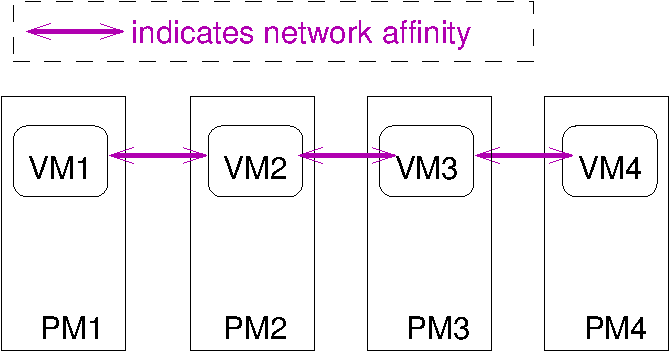
\includegraphics[scale=0.6]{arescue-figures/mutable-immutable.pdf}}
	~~~~~~~~~~~~~~~~~~~~~~~~~~
	\subfloat[VM3 migrates to PM2]{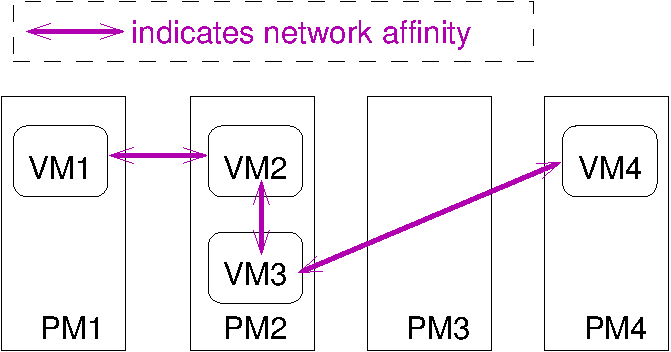
\includegraphics[scale=0.6]{arescue-figures/mutable-immutable-2.pdf}}
	\caption{Example to demonstrate \textit{mutable} and \textit{immutable} network affinity.}
\label{fig:mutable}
\end{center}
\end{figure}

In the initial state (refer Fig.~\ref{fig:mutable}(a)), all VMs are
hosted on different PMs (i.e. dispersed), hence the network traffic
in each case is \textit{inter-PM}. Suppose VM3 is now migrated from
PM3 to PM2, it gets colocated with VM2, resulting in the 
configuration shown in Fig.~\ref{fig:mutable}(b). 
After the migration, the nature of traffic between VM2 and VM3
has changed from \textit{inter-PM} to \textit{intra-PM}, whereas VM2
continues to have \textit{inter-PM} network affinity with VM1.
Thus, migration of VM2 caused its network traffic with VM3 to 
change nature, while its traffic with VM1 remained unchanged. We differentiate
these two types of network traffic as \textit{mutable} and \textit{immutable}
network traffic.
Basically, for a given VM migration, \textit{mutable} network traffic 
is that which changes nature between \textit{inter-PM} and \textit{intra-PM},
and \textit{immutable} network traffic is that whose nature does not change
due to migration.

We present benchmarking experiments
which demonstrate impact due to network affinity
on CPU usage of virtual machines and their hosts, when communicating
VMs are colocated as compared to when they are dispersed. 
Motivated by the benchmark findings, we develop models
that can estimate the ``colocated'' CPU resource usage when VMs transition
from dispersed placements to colocated, and can estimate the ``dispersed''
CPU resource usage when VMs transition from colocated placements to dispersed. 
These models predict CPU usage in target
scenario (colocated/dispersed) based on resource usage profiles
from source scenario (dispersed/colocated).

Initially we built models to predict total CPU usage for target scenario,
based on all resource usage profiles like CPU, disk, mutable network
and immutable network usage. However, the maximum error with these
predictions was found to be around 4 to 6\% absolute CPU usage.
Consequently, based on our findings that CPU usage is affected only by
\textit{mutable} network traffic levels, we built models to
predict the difference in CPU usage based on only
the mutable network traffic profiles. These models were much more
accurate, with maximum error within 2\%. Finally, we applied these
pair-wise models to multi-VM scenarios using a multi-phase
prediction methodology. This demonstrated that simple models
built on the scale of two VMs could be successfully used to
predict for multi-VM scenarios as well.
%In our work, we perform empirical quantification of 
%the CPU resource that Xen-based VMs would require if they were
%to be migrated for colocation or dispersion (splitting up of 
%previously-colocated VMs). 
%
%We are concerned with CPU utilization required to handle network
%In Xen virtualization environment, a
%privileged virtual machine (called Domain-0 or 
%Dom0\index{Dom0}\nomenclature{Dom0:}{Privileged domain or privileged virtual 
%machine or Domain-0}) manages network 
%traffic for the guests (called User Domain or 
%DomU\index{DomU}\nomenclature{DomU:}{User domain or Domain-U})
%and utilizes CPU proportional to network traffic volume.
%In this work, we explore the effect of
%network-affinity on CPU usage of colocated and dispersed VMs. More
%specifically, \textit{what is the effect on CPU utilization of mutually
%communicating VMs based on whether they are colocated or dispersed?}
%An important consideration for migration and consolidation related
%decisions is the expected resources required for the VM
%on the target machine. The consolidation of
%VMs into a colocated set and the migration of VMs to dispersed
%placements, can result in different CPU resource requirements.
%The focus of the first component of this thesis, is to build
%\emph{affinity-aware} models that can predict expected CPU
%resource requirements\textemdash{}upon colocation or dispersion of VMs.
Our contributions are,
\begin{enumerate}	
\item \emph{Event profiling} of intra-PM and inter-PM network
	communication paths in Xen, using \texttt{Xenoprof}~\cite{xenoprof}.
\item \emph{Benchmark} CPU resource requirements
of VMs with different levels of network-affinity
in colocated and dispersed configurations.
\item Perform the above benchmarking step for both Xen and KVM virtualization environments,
	showing that a linear relationship between network usage and the resulting CPU overhead
	exists in both.
\item Develop \emph{pair-wise affinity-aware} models to predict \textit{total}
	as well as \textit{differential} CPU usage, when a pair of VMs move between
	dispersed and colocated placements.
\item Apply above pair-wise models to \emph{multi-VM scenarios}, where
	a single migrating VM has more than one neighboring
	VMs with which it exhibits network-affinity, both on source \& target PMs.
\item Present a \emph{comprehensive evaluation} using synthetic 
	workloads \& benchmark applications,
	of the models as well as application to multi-VM scenarios.
\end{enumerate}

\noindent The rest of this chapter is structured as follows. 
Section~\ref{sec:arescue-background}
presents background regarding network virtualization in Xen and KVM, and
problem statement is presented in Section~\ref{sec:arescue-problem}.
Section~\ref{sec:arescue-benchmark}
presents empirical benchmarking of the effects of relative placement on
CPU usage of communicating VMs, in both Xen and KVM virtualization environments.
Section~\ref{sec:arescue-our-approach} presents our approach to
build affinity-aware models to predict CPU usage for Xen DomU and Dom0
and Section~\ref{sec:arescue-experimental-eval} presents evaluation 
of the models.
Section~\ref{sec:arescue-related-work} presents related work in juxtaposition
with our work and 
in Section~\ref{sec:arescue-open-directions}, we
present our ideas for future work.
%in the area of affinity-aware CPU usage modeling and 
Section~\ref{sec:arescue-conclusions} concludes the chapter.


\label{sec:arescue-intro}

\section{Background}
\label{sec:arescue-background} This section recalls the concept of network I/O
virtualization in Xen\index{Xen} and KVM\index{KVM} 
(previously presented in detail in
Section~\ref{sec:litreviewchap-io-virtualization}), and supplements it
with an event profiling study of network virtualization in Xen.

\subsection{Recalling the basics of network I/O virtualization}
As discussed in Chapter~\ref{chap:thesis-litreview}, network I/O 
virtualization technologies are:
\begin{enumerate}
\item Para-virtualization based driver domain I/O model,
\item Emulation-based direct I/O model and
\item Virtio-based split-driver I/O model
\end{enumerate}
Note that, both the driver domain I/O model and the virtio model 
have the concept of a split-driver, with the difference
that virtio can be used even in para-virtualization setups, eg Xen.
A split-driver architecture consists of
\texttt{frontend} and \texttt{backend} drivers, of which the 
\texttt{backend} driver is responsible to communicate with 
native network drivers and get the I/O performed on behalf of 
virtual machines. 

An in-depth survey of various shared-memory optimizations
for inter-virtual-machine (i.e. intra-PM) communication
is presented in \cite{shared-mem-optimizations}---and it
presents optimizations in both the para-virtualization
and emulation-based-virtualization setups.
In all above cases, for network communication between VMs 
colocated on a single PM, the native driver 
does not need to be invoked at all whereas
if VMs are hosted on different PMs, physical network
communication is essential. 
This difference manifests as different
CPU overheads for the VMs and the physical hosts 
concerned. In this section, 
we present an event profiling study of CPU overheads in both scenarios,
in the Xen paravirtualization setup.

\subsection{Profiling study of network I/O virtualization}
% Xen uses an inter-domain shared memory mechanism to share data between
% colocated VMs. 
To further motivate the study of differences in communication between
colocated and dispersed virtual machines, we performed a detailed 
profiling-based study of Xen's\index{Xen} 
networking architecture and 
implementation~\cite{xen-internals, xen-networking, linux-networking}. 
% The major difference between dispersed
% and colocated communication is that 

A common optimization in the network communication in colocated case is that 
packet check-summing
(both calculation and verification) is not performed since it is assumed 
that memory copying (performed in colocated case) is quite reliable as 
opposed to physical network transmission (corresponding to dispersed case). 
Additionally, when Xen-based VMs are colocated, they are
connected via a layer 2 software bridge and hence a packet 
transmitted from one VM to another colocated VM is locally delivered 
on the bridge itself. On the other hand, when communicating VMs 
are on different PMs, a packet transmission by one VM
is forwarded over the software bridge, 
DMA-copied\nomenclature{DMA:}{Direct Memory Access}\index{DMA}
into the network interface 
card's (NIC\nomenclature{NIC:}{Network Interface Card}\index{NIC}) 
buffer, and placed on the network link by the NIC. This
transmitted packet is then received on the destination host's NIC, 
copied into a kernel buffer for further processing
and interrupt sent to destination host's driver domain (Dom0). Upon
subsequent scheduling, the received packet is inspected by Dom0 to
determine the destination VM, packet delivery is scheduled and destination 
VM is notified of incoming packet. Thus, end-to-end communication
path in dispersed case is comparatively longer than in colocated case.

Using the tool \texttt{Xenoprof}~\cite{xenoprof}, we performed
event monitoring for network transmission between a pair of Xen-based 
VMs in both colocated and dispersed scenarios. 
\texttt{Xenoprof} performs statistical profiling of applications
using non-maskable interrupts when a performance counter overflows,
to sample the function under execution. Since it
performs statistical sampling, higher number of samples 
of a specific function call can imply either that a
single invocation of the function had a long execution 
time compared to other functions, 
or that the function call had higher
number of invocations as compared to others, or both.

To perform the profiling study, 
TCP\nomenclature{TCP:}{Transport Control Protocol}\index{TCP}
network traffic of
50Mbps was generated from one VM to the other,
%using application-level packet size (henceforth referred to as \textit{segment size}\index{segment size}) of 30KB 
wherein VM1 sent requests for a certain number of bytes, 
and VM2 served the requests
by transmitting back the requested number of bytes. 
It may be noted that neither of the VMs are pure transmitters
or pure receivers\textemdash{}because VM1 (i)~sends requests, (ii)~receives responses
and (iii)~sends TCP acknowledgements whereas VM2 (i)~receives requests and
(ii)~sends responses.
However, we define the VMs as being ``transmitting'' and ``receiving'' 
in terms of the direction of data traffic,
i.e., the VM sending requests receives data responses, 
hence is the \emph{receiver},
whereas the VM receiving requests sends data responses and 
is the \emph{transmitter}.
Thus, in our example, VM2 is the transmitter (of requested data) and 
VM1 the receiver (of requested data). 
We refer to Dom0 on VM2's host as the transmitting Dom0 
and the Dom0 on VM1's host as the receiving Dom0. 
%Since we wished to analyze TCP communication 
%overheads, such bi-directional communication flows were unavoidable. 

We perform monitoring on both the transmitting Dom0 (\textit{Disp-Tx})
and the receiving Dom0 (\textit{Disp-Rx}) in the dispersed case. 
Meanwhile in the colocated case, we perform monitoring on the 
sole Dom0\index{Dom0}
instance (\textit{Colo}) which performs both transmit and receive processing.
Our aim is to empirically observe the 
difference in CPU processing required in the three cases
\textemdash{}(i)~\textit{Disp-Tx} (short for Dispersed-Transmit), 
(ii)~\textit{Disp-Rx} (short for Dispersed-Receive) and 
(iii)~\textit{Colo} (short for Colocated).
We consider the 10 most sampled function calls in each case.
Since we are interested in the differences and not the similarities, hence
we discard those calls which are common to all three lists. 
We compute the union of all three lists and select those function
calls that exhibit some distinctive feature of network flow.
The sample counts of these calls are enumerated in Table 
\ref{tab:xenoprof-30KB-norm} for all the three
cases.
% present
% the number of samples reported by Xenoprof for those function
% calls which have distinctive behaviour in Table \ref{tab:xenoprof-30KB-norm}. 
% To make the numbers more coherent to understand, we present in
% Table \ref{tab:xenoprof-30KB-norm} 
The number of samples is represented in a
normalized format, wherein for every function call, the number
of calls in each of the three cases is normalized w.r.t the
case which
has the highest number of samples. For example, the function
\texttt{change\_page\_attr} has highest number of samples
in \textit{Disp-Rx} case and almost negligible numbers in the other
cases. The normalized number is shown correct to 2 decimal 
places, so very low numbers get automatically rounded off to 0,
thus further simplifying our analysis. Thus, the function calls
that are listed as having 0.0 samples are those which have very 
few samples in the \texttt{Xenoprof} output.


% \begin{table}[t]
% \centering
% % \noindent\makebox[\textwidth]{%
% \begin{tabular}{|c|c|c|c|} \hline
% \textbf{Function} & \multicolumn{3}{|c|}{\textbf{Number of samples}} \\ \cline{2-4}
% \textbf{Call} & \textbf{Disp-Tx} & \textbf{Disp-Rx}  & \textbf{Colo} \\ \hline  
% \texttt{/e1000} & 209997 & 242202 & 2311 \\
% \texttt{/bridge} &	130362 & 154456 & 114009 \\
% \texttt{change\_page\_attr} & 229 & 94889 & 384 \\
% \texttt{x86\_emulate} & 202 & 89053 & 372  \\
% \texttt{flush\_area\_local} & 25179 & 121486 & 21910 \\
% \texttt{\_\_copy\_from\_user\_ll} & 23449 & 116011 & 25519 \\
% \texttt{evtchn\_set\_pending} & 28233 & 63585 & 26638 \\
% \texttt{evtchn\_do\_upcall} & 26278 & 46489 & 23753 \\
% \texttt{nf\_iterate} & 35678 & 40846 & 32485 \\
% \texttt{\_spin\_unlock\_irqrestore} & 50895 & 60517 & 49261 \\
% \texttt{net\_rx\_action} & 42467 & 77225 & 54090 \\
% \texttt{do\_grant\_table\_op} & 35344 & 55089 & 65292 \\
% \texttt{get\_page} & 14742 & 35037 & 53635 \\
% \texttt{\_\_acquire\_grant\_for\_copy} & 9565 & 24982 & 38502  \\
% \texttt{gnttab\_copy} & 10446 & 90687 & 160845 \\
% \texttt{\_\_release\_grant\_for\_copy} & 7692 & 15693 & 42386 \\ \hline
% \end{tabular}
% % }
% \caption{Comparison of number of samples reported by Xenoprof monitoring}
% \label{tab:xenoprof-30KB}
% \end{table}

% \begin{table}[t]
% \centering
% % \noindent\makebox[\textwidth]{%
% \begin{tabular}{|c|c|c|c|} \hline
% \textbf{Function} & \multicolumn{3}{|c|}{\textbf{Normalized num of samples}} \\ \cline{2-4}
% \textbf{Call} & \textbf{Disp-Tx} & \textbf{Disp-Rx}  & \textbf{Colo} \\ \hline  
% \texttt{change\_page\_attr} & 0.00 & 1.00 & 0.00    \\
% \texttt{x86\_emulate} & 0.00 & 1.00 & 0.00 \\
% \texttt{flush\_area\_local} & 0.21 & 1.00 & 0.18   \\
% \texttt{\_\_copy\_from\_user\_ll} & 0.20 & 1.00 & 0.22 \\
% \texttt{evtchn\_set\_pending} & 0.44 & 1.00 & 0.42 \\
% \texttt{evtchn\_do\_upcall} & 0.57 & 1.00 & 0.51    \\
% % \texttt{nf\_iterate} & 0.87 & 1.00 & 0.80  \\
% % \texttt{\_spin\_unlock\_irqrestore} & 0.84 & 1.00 & 0.81 \\
% % \texttt{net\_rx\_action} & 0.46 & 0.71 & 0.85 \\
% % \texttt{do\_grant\_table\_op} & 0.54 & 0.84 & 1.00  \\
% \texttt{get\_page} & 0.27 & 0.65 & 1.00   \\
% \texttt{\_\_acquire\_grant\_for\_copy} & 0.25 & 0.65 & 1.00    \\
% \texttt{gnttab\_copy} & 0.06 & 0.56 & 1.00 \\
% \texttt{\_\_release\_grant\_for\_copy} & 0.18 & 0.37 & 1.00 \\ \hline
% \end{tabular}
% % }
% \caption{Normalized number of samples reported by Xenoprof monitoring}
% \label{tab:xenoprof-30KB-norm}
% \end{table}

\begin{table}[t]
\caption{Normalized number of samples reported by Xenoprof}
\label{tab:xenoprof-30KB-norm}
\centering
\vspace{0.1in}
% \noindent\makebox[\textwidth]{%
\begin{tabular}{|c|c|c|c|} \hline
\textbf{Function} & \multicolumn{3}{|c|}{\textbf{Normalized num of samples}} \\ \cline{2-4}
\textbf{Call} & \textbf{Disp-Tx} & \textbf{Disp-Rx}  & \textbf{Colo} \\ \hline  
\texttt{\/e1000} & 0.87 & 1.00 & 0.01 \\
\texttt{gnttab\_copy} & 0.06 & 0.56 & 1.00 \\
\texttt{\/bridge} & 0.84 & 1.00 & 0.74 \\
% \texttt{flush\_area\_local} & 0.21 & 1.00 & 0.18 \\
% \texttt{\_\_copy\_from\_user\_ll} & 0.20 & 1.00 & 0.22 \\
\texttt{change\_page\_attr} & 0.00 & 1.00 & 0.00 \\
\texttt{x86\_emulate} & 0.00 & 1.00 & 0.00 \\ 
\texttt{do\_mmuext\_op} & 0.00 & 1.00 & 0.01 \\
%\texttt{ptwr\_emulated\_update} &  0.00 & 1.00 & 0.00 \\
\texttt{ptwr\_do\_page\_fault} &  0.00 & 1.00 & 0.00 \\
\texttt{get\_page\_from\_l1e} &  0.00 & 1.00 & 0.00 \\
\texttt{xen\_tlb\_flush} &  0.00 & 1.00 & 0.00 \\ 
All & 0.44 & 1.00 & 0.49 \\ \hline
\end{tabular}
% }
\end{table}

\paragraph{Observations from profiling study.}
From Table \ref{tab:xenoprof-30KB-norm}, we make the following 
observations,
\begin{itemize}
\item \texttt{e1000} (the native network driver) is used only 
in the dispersed case whereas in the colocated case, network packets are passed 
from source to destination over the bridge without using the native driver.
\item \texttt{gnttab\_copy} is a page copy mechanism involving grant
tables. Hence, it is used significantly in \textit{Disp-Rx} for copying packets
from Dom0 memory to the receiving DomU and the highest in \textit{Colo}
case where Dom0 copies the packet from the transmitting DomU to 
the receiving DomU\index{DomU}. It is not used much in \textit{Disp-Tx} 
because of scatter/gather wherein the data to be transmitted is 
collected by DMA\index{DMA} device directly from DomU memory. 
\item \texttt{bridge} is used approximately equally in all three cases. 
This is because packet delivery in colocated case needs a one-shot
traversal of the bridge as compared to traversing the bridge on both
transmitting and receiving ends in the dispersed case.
\item \texttt{change}\_\texttt{page}\_\texttt{attr}, 
\texttt{ptwr\_do\_page\_fault}, \\
\texttt{get}\_\texttt{page}\_\texttt{from}\_\texttt{l1e},
\texttt{xen\_tlb\_flush},
\texttt{x86\_emulate}
\& \texttt{do\_mmuext\_op}
are related to the copying of
received packets from the network buffer to Dom0\index{Dom0}
memory, wherein Dom0 has to acquire free pages, request for copying
of packets to those free pages, and facilitate guest TLB updates.
%using writable page tables approach.
% (\texttt{ptwr\_*}). Thus, 
These calls, being specific to dispersed receive flow, are absent in
colocated case network flow.
\end{itemize}
Thus, depending on whether the VMs are colocated
(causing intra-PM network traffic), 
or dispersed (causing inter-PM network traffic), 
the network communication between them follows
different data-paths, in-turn incurring different overheads.
These differences in CPU overheads were observed empirically with both 
Xen and KVM environments (presented in Section~\ref{sec:arescue-benchmark}). 
%as presented in subsequent sections.

 

\section{Problem definition}

We are interested in the problem of estimating the %average
CPU utilization of a virtual machine, based on its location relative
to its communicating set of virtual machines.
% when being
% considered for consolidation or migration to a target PM. 
Additionally, the virtual machine should be
able to continue execution of its tasks to meet
specified service level objectives.
% As we demonstrate (in Section \ref{tnsm-benchmark}),
Since CPU is the primary resource affected due to handling network I/O
operations in colocated and dispersed scenarios, the scope of this work 
is restricted to predicting CPU resource usage.

We consider the following scenario for our problem.
A set of applications, each application having several mutually
communicating components or tiers, are
provisioned as VMs in a cluster of inter-connected PMs.
Thus, each VM has network activity, disk activity and CPU utilization. 
Since disk partitions may be 
network-attached (NFS-mounted\nomenclature{NFS:}{Network File System}\index{NFS} or 
SAN\nomenclature{SAN:}{Storage Area Network}\index{SAN} or
NAS\nomenclature{NAS:}{Network-attached Storage}\index{NAS} appliance), disk activity of
guest VMs\index{VM} may also manifest as network traffic at their host PM\index{PM}.
In this setting,
pro-actively or reactively, a decision process may decide
to move/migrate a subset of VMs to meet dynamic resource
requirements or to consolidate VMs on fewer PMs,
and a vital input to this decision process
is the resource requirements of the VM on the target machine
after migration.

Given a set of virtual machines and their current resource utilization 
levels, our aim is to predict CPU resource required by 
the virtual machine on target host after migration. Additionally,
the virtual machine should be able 
to support the \emph{same load level} as on the source physical machine.
Memory is assumed to be not a bottleneck in our placement configurations,
and the VMs are assumed to maintain their intrinsic resource
utilization levels towards maintaining the SLA guarantees.

In~\cite{virtual-putty}, there is allusion to the possibility 
of change in resource requirements upon a change in the
hosting scenario of two communicating VMs\textemdash{}however, 
empirical quantification is lacking. As part of our work,
we perform a detailed benchmarking exercise to empirically 
demonstrate that there is indeed a difference in CPU utilization of
communicating VMs when their hosting scenario changes between
\textit{colocated} and \textit{dispersed}. The difference in CPU usage for
intra-PM (due to VM colocation) and inter-PM (due to VM dispersion)
network communication forms the motivation for
affinity-aware CPU usage modeling.
% estimating the CPU requirement upon migration. 
Benchmarking for both Xen and KVM virtualization environments is presented 
in the next section and 
% when the current CPU usage and other resource usage
% profiles are known, is that intra-PM (due to colocation) and 
% inter-PM (due to dispersion) network
% communication incur different overheads (as already discussed
% in Section \ref{tnsm-intro}).
% Each VM's CPU utilization is characterized by its
% own CPU usage (CPU utilized by DomU), its affine and non-affine
% network traffic, and its disk read/write activity.
% Dom0 CPU utilization occurs on account of the guest or application
% VM's disk and network
% I/O, and is characterized by the hosted VMs' resource usages.
% Based on whether the VMs are being consolidated or separated
% out, the net CPU usage will decrease or increase.
towards CPU requirement prediction, we build models for both the 
colocation and dispersion scenarios, which we describe in detail 
in the following sections.

\label{sec:arescue-problem}

\section{Benchmarking with colocated and dispersed provisioning}
In this section, we study the implications of 
communication among VMs in colocated and dispersed 
placement scenarios. 
Although the study reveals that there are differences in CPU
utilization based on the placement scenarios, however the exact
CPU utilization levels are incidental to (i) the operating system
versions, (ii) the virtualization technology used and its version,
(iii) the physical machines used and their configurations.
%, and hence
%we do not claim generality in terms of their quantifications.


\subsection{Experimental setup}
\label{sec:arescue-setup}

\begin{figure}[t]
\centering
\subfloat[Xen setup]{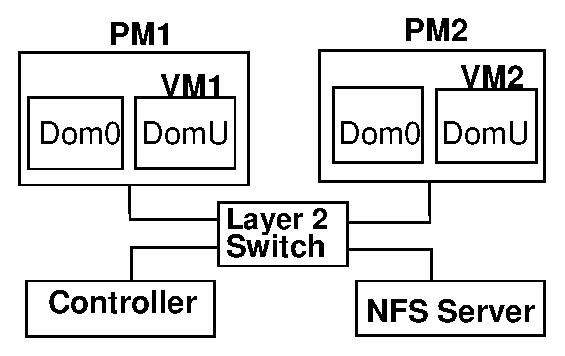
\includegraphics[scale=0.695]{jss-figures/benchmark}} 
~~~~~~~~~~~~~~~~~~~~
\subfloat[KVM setup]{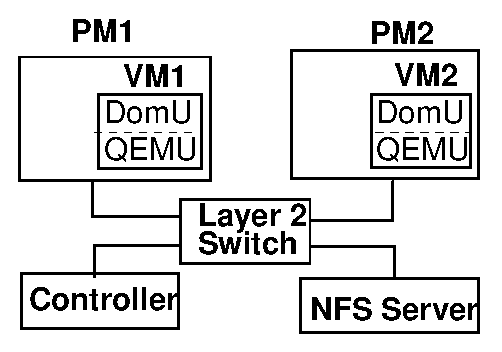
\includegraphics[scale=0.695]{jss-figures/kvmbenchmark}}
\caption{Setup for benchmarking, profiling and model evaluation.}
\label{fig:setup}
\end{figure}
Fig.~\ref{fig:setup} shows the experimental setup that we used. 
The setup used for benchmarking with Xen virtualization technology
is as shown in Fig.\ref{fig:setup}(a) wherein Dom0 is the privileged
domain as described earlier in Section~\ref{sec:litreviewchap-io-virtualization}. 
In case of KVM platform, 
there is no management domain since it
does not follow the driver domain I/O model. Hence, the setup
for KVM benchmarking is a slightly modified version, as
depicted in Fig.~\ref{fig:setup}(b).

As shown in the setup of Fig.~\ref{fig:setup}, two PMs (both with same 
configurations) host the VMs. Each PM
is connected via a Layer-2 Switch to an NFS server which hosts
disk images associated with the VMs. Thus, all disk read/write
operations are NFS-read/write operations which generate network traffic
at the host. The Controller is responsible
for coordination of load generation and resource-usage measurements 
on the VMs.
Load generation is done using an automated script residing at the Controller,
that invokes a custom application program (called \texttt{LoadGen})
at each VM.
For logging of resource utilization, we adopt the ``black-box''
approach~\cite{sandpiper}, i.e, we monitor VM's resource usage by measuring 
only at the hosts (PMs) and not inside the VMs.
% and not within the VMs themselves.
Resource utilization logging is done on the host, using utilities like
\texttt{sar}~\cite{sar}, \texttt{Xentop}~\cite{xentop} (for Xen), 
\texttt{top}~\cite{top} (for KVM) and 
\texttt{iptables}~\cite{iptables}.

The two physical machines hosting the VMs are Intel Core 2
Quad (Q9550) machines with 2.83 GHz cores. Xen version is
3.2 with Linux kernel 2.6.24-26 and KVM version is kvm-62
having QEMU PC emulator version 0.9.1.
%  and are dual-booting
% with Xen 3.2 virtualization environment and KVM module installed in Linux
% kernel version 2.6.24-26.
Both Controller and NFS server (not virtualized, hence common to 
both Xen and KVM setups) are Intel Core 2 (E7400) machines with 
2.60 GHz cores.
The Layer-2 Switch and all network links of the
machines operate at 100 Mbps.


\subsection{Workload generation}
\label{sec:arescue-workloadgen}
As part of our experimental evaluation, we generate 
different types of workloads for benchmarking and
model building.
Workloads are generated using a generic client-server setup,
wherein a \textit{client}
(the controller machine) remotely connects to 
the \textit{servers} (each PM or Dom0,
and VM or DomU). % where workload is to be generated. 
The workload generation
tool resides on each such ``server'' and complies with the 
load generation
requests received from the ``client'' machine. 
Referring to Fig.~\ref{fig:setup}, the 
workload generation requests are sent by the ``Controller''
and VM1/VM2 execute benchmarks to generate the 
requested resource utilization levels. 

Though more detail regarding the design, implementation
and usage of the load generation tool (called \texttt{LoadGen})
is presented in Appendix~\ref{chap:thesis-loadgen}, here 
we mention the different workloads briefly.
The different types of workloads generated by \texttt{LoadGen} are,
% 
% \textbf{SSS:Write up about micro-benchmarks. Also, mention
% the exponential number of cases to consider for combinational loads, and hence
% the randomized choice of combinational load cases.}
\begin{itemize}
\item \textbf{CPU-intensive workloads.}
CPU intensive workloads are generated by having a worker
thread calculate a Fibonacci series with varying periodicity.
If $T$ is the average time for a round of Fibonacci series calculation,
CPU load of $X\%$ is generated by having the worker thread perform
computations for $X \times T$ milliseconds (\emph{active period}) and
sleep for ($100-X) \times T$ milliseconds (\emph{sleep period}).
\item \textbf{Mutable and immutable network-intensive workloads.} 
We generate various levels of network traffic between a pair of VMs by using
a TCP-based custom application that sends a string of bytes on a
TCP socket with different periodicity.
For network workloads, we assume the maximum available capacity 
to be $100$ Mbps and vary the load on each VM by steps 
of $10$ Mbps, from $10$ to $90$ Mbps.
\item \textbf{Disk read \& write workloads.}
We generate disk read (or write) workload by reading (or writing) files  
of $4 kB$ size, with varying intervals to achieve different read access
rates ranging from 0 to 1280 blocks/second. Translating into Kbps, these
rates range from 0 to 5120 Kbps.
\item \textbf{Combination workloads.}
Combination or mixed workloads are generated using 
the same procedures as described above, with a 
multi-threaded process executing different workloads 
simultaneously.
\end{itemize}
As part of the experimental setup, we ensured that for each 
experiment, all combinations of workloads over all VMs do not 
saturate capacity of any resource, i.e., CPU utilization and 
I/O utilization levels are always less than 100\% in all experiments.

\subsection{Effect of colocation on CPU usage}
In this section, we empirically observe the effect of colocation
on CPU resource usages of both Dom0 and DomU. 
By design, we generate the ``same'' load (type and 
amount) for each experiment in both the configurations\textemdash{}dispersed and 
colocated\textemdash{}and observe the differences in actual resource utilization
levels. 
We are interested in addressing the following questions,
(i) For mutable network workloads, is there a decrease in CPU usage when
VMs are colocated, as compared to when they are dispersed? 
(ii) For pure CPU-intensive workloads, is the colocated Dom0 CPU usage
a simple summation of the individual (or dispersed) Dom0 usages, (iii) For
disk read \& write workloads, and immutable network workloads, is
the resultant colocated CPU usage a summation of usages in dispersed
scenarios?

%\begin{figure}%
%\hspace{-0.3in}
%\subfloat[DomU CPU utilization for Rx]{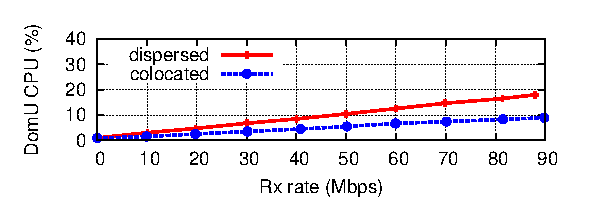
\includegraphics[scale=0.9]{arescue-figures/aff-benchmark/domU-cpu-vs-affine-rx-curve.eps}}
%\subfloat[DomU CPU utilization for Tx]{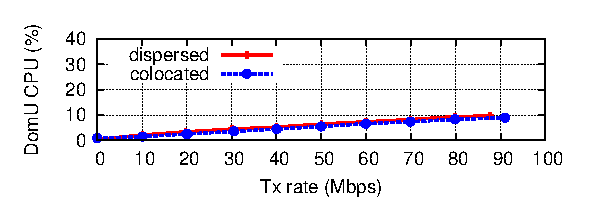
\includegraphics[scale=0.9]{arescue-figures/aff-benchmark/domU-cpu-vs-affine-tx-curve.eps}} \\
%\centering
%\subfloat[Dom0 CPU utilization for Rx/Tx]{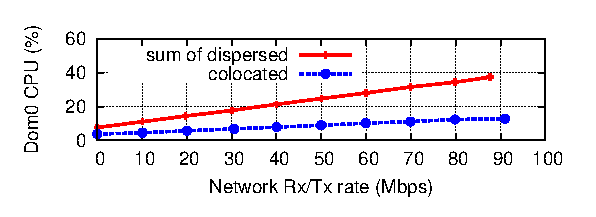
\includegraphics[scale=0.9]{arescue-figures/aff-benchmark/dom0-cpu-vs-affine-curve.eps}}%
%\caption{CPU utilization due to intra-PM network traffic (in Xen setup).}
%\label{fig:cpuovhd-rxtx}
%\end{figure}

%from 2ndchap-benchmark.tex
\begin{figure}[t]%
	% \centering
	\hspace{-0.3in}
	\subfloat[Dispersed DomU CPU utilization for Tx]{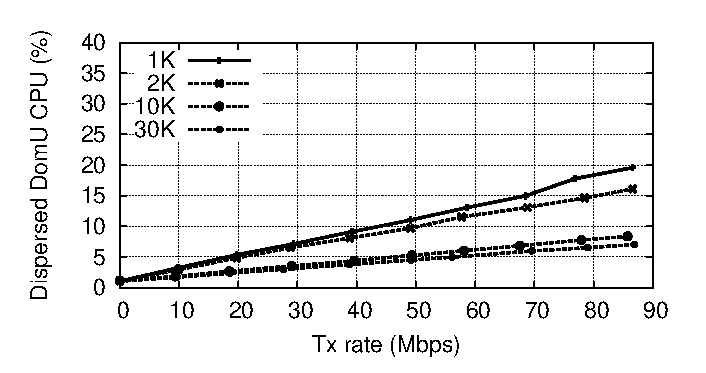
\includegraphics[scale=0.75]{jss-figures/new-aff-benchmark/domu-disp-cpu-for-tx-diff-file-sizes-notsoboth.eps}} ~~
	\subfloat[Colocated DomU CPU utilization for Tx]{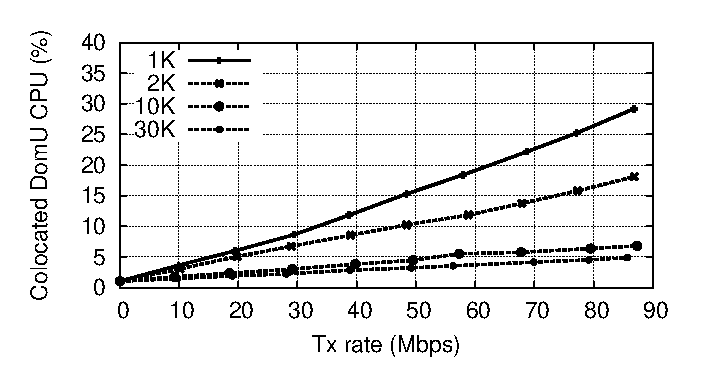
\includegraphics[scale=0.75]{jss-figures/new-aff-benchmark/domu-colo-cpu-for-tx-diff-file-sizes-notsoboth.eps}}
	\caption{CPU utilization due to mutable transmit traffic in dispersed and colocated scenarios with different segment sizes (in Xen setup).}
	\label{fig:xendomutx-chunks}
\end{figure}

\begin{figure}%
	% \centering
	\hspace{-0.3in}
	\subfloat[Dispersed DomU CPU utilization for Rx]{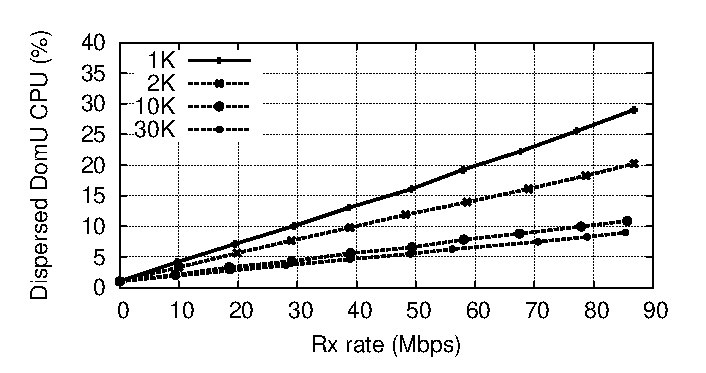
\includegraphics[scale=0.75]{jss-figures/new-aff-benchmark/domu-disp-cpu-for-rx-diff-file-sizes-notsoboth.eps}} ~~
	\subfloat[Colocated DomU CPU utilization for Rx]{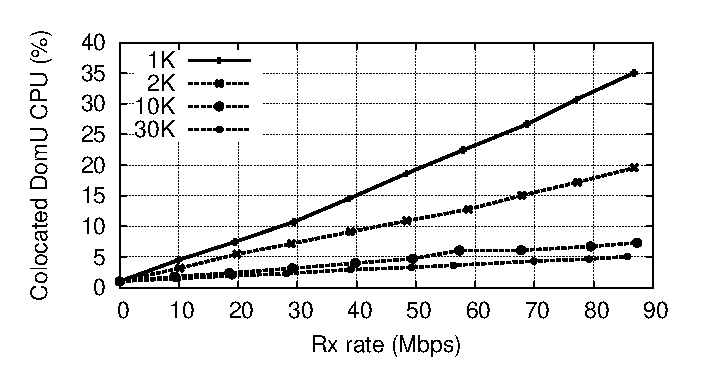
\includegraphics[scale=0.75]{jss-figures/new-aff-benchmark/domu-colo-cpu-for-rx-diff-file-sizes-notsoboth.eps}}
	\caption{CPU utilization due to mutable receive traffic in dispersed and colocated scenarios with different segment sizes (in Xen setup).}
	\label{fig:xendomurx-chunks}
\end{figure}

\begin{figure}[t]
	% \centering
	\hspace{-0.3in}
	\subfloat[Dispersed summation Dom0 CPU utilization for Rx/Tx]{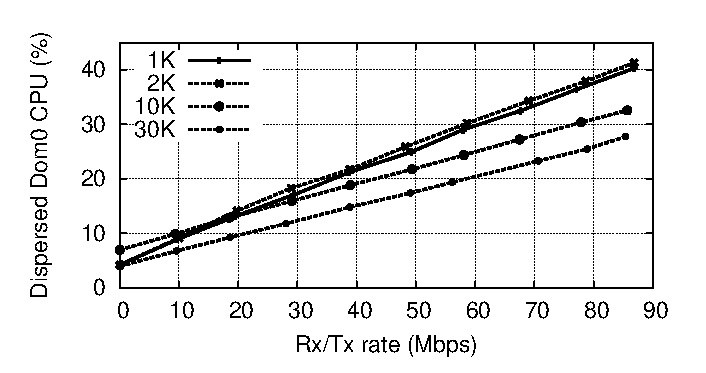
\includegraphics[scale=0.75]{jss-figures/new-aff-benchmark/dom0-dispsum-cpu-for-rxtx-diff-file-sizes-notsoboth.eps}} ~~
	\subfloat[Colocated Dom0 CPU utilization for Rx/Tx]{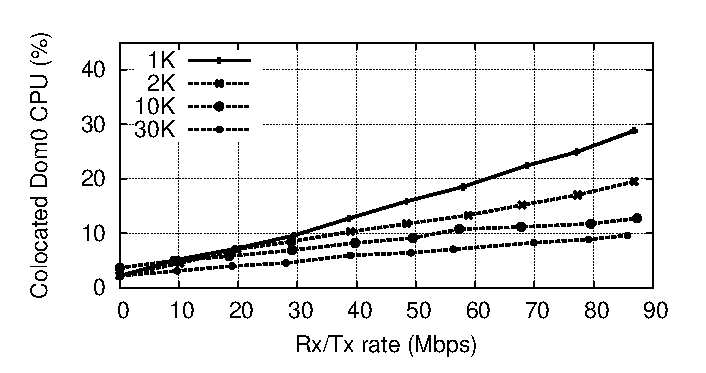
\includegraphics[scale=0.75]{jss-figures/new-aff-benchmark/dom0-colo-cpu-for-rxtx-diff-file-sizes-notsoboth.eps}}
	\caption{CPU utilization for mutable network traffic with different segment sizes (in Xen setup).}
	\label{fig:dom0rxtx}
\end{figure}

\paragraph{I. Impact of mutable network traffic in Xen.} 
One of our claims (and as also discussed 
in~\cite{virtual-putty}, \cite{starling}),
is that colocated provisioning can result in changes in
resource usage for mutually communicating VMs. % and availability. 
% `Affine' traffic refers to the network communication
% within the VM pair under consideration.
In this experiment, VM1
and VM2 act as a Tx/Rx pair to transmit and receive data
at different rates, such that
VM1 is the transmitting DomU\index{DomU}
and VM2 is the receiving DomU.
To study the implications of mutable network-affinity
between VMs, the experiment is conducted in both 
colocated and dispersed scenarios, and CPU utilization for
DomU (and Dom0 in Xen) is measured.
In our setup, we observed that TSO (TCP Segmentation
Offload)\nomenclature{TSO:}{TCP Segmentation Offload}\index{TSO} feature was
enabled whereas the complementary feature LRO (Large
Receive Offload)\nomenclature{LRO:}{Large Receive Offload}\index{LRO} at
receiving end
was not functional. For the sake of
uniformity at both transmitting and receiving ends, we disabled
TSO for our experiments.

Fig.~\ref{fig:xendomutx-chunks}(a) and \ref{fig:xendomutx-chunks}(b)
plot the transmitting DomU's CPU utilization for varying usage
of network bandwidth in Xen\index{Xen} setup. Each line represents
the use of a different application-level segment size
(sizes are mentioned in the legend).
As described in Section~\ref{sec:arescue-background}, inter-PM and
intra-PM communication have different execution paths,
hence resulting in different CPU utilization.
As can be seen, for higher segment sizes, increase
in network bandwidth usage results in higher CPU savings upon
colocation. However, the opposite result is
observed for smaller segment sizes.
The bold lines in the graph represent those
segment sizes for which colocated CPU usage is higher than
dispersed whereas the dotted lines indicate those having
colocated CPU usage as lower than dispersed. For example,
for the segment size of 30KB at 80Mbps network utilization,
CPU utilization is 8\% for dispersed and 4.8\% for colocated,
thus indicating a drop of approximately 3\% absolute CPU
when transitioning into colocated. On the other other hand,
for the segment size of 1KB at 85Mbps, CPU utilization
is 29\% for dispersed and 35\% for the colocated scenario,
which indicates a 6\% increase while moving into colocated placement.
A similar result was observed for the receiving DomU as well,
as depicted in Fig.~\ref{fig:xendomurx-chunks}.

Fig.~\ref{fig:dom0rxtx} shows Dom0 CPU utilization
levels for two communicating VMs,
with
\ref{fig:dom0rxtx}(a)
showing the summation of the two dispersed Dom0 CPU utilization
and
\ref{fig:dom0rxtx}(b)
showing the colocated Dom0 utilization.
We can see that in all cases,
the summation utilization is significantly greater than the
colocated Dom0 utilization. For example,
for the segment size of 30KB at 80Mbps network utilization,
the difference in absolute Dom0 CPU usage between
dispersed (summation of utilization at both Dom0's in the
dispersed scenario) and colocated (single
Dom0 CPU) scenarios is 16\% and similarly for 2KB segment size,
this difference is around 20\% absolute CPU.
The above observations suggest that not only the bit-rate of
transmission, but also the segment size affects CPU utilization
in both colocated and dispersed scenarios, and we need to consider
both these factors while modeling CPU usage. Further, we also
observe that in all above experiments, CPU usage varies linearly
with respect to network utilization.


% This implies that there is definitely
% no increase in CPU utilization due to colocation of two 
% communicating VMs.
%Further, the absolute usage by Rx-network traffic is more
%than Tx-traffic for the same bandwidth\textemdash{}CPU utilization
%of 17\% and 9\% respectively, at 90 Mbps network bandwidth
%utilization.
%Fig.~\ref{fig:cpuovhd-rxtx}(c) shows the Dom0 CPU utilization
%levels for two communicating VMs.
%Comparing network rates of 40 Mbps and 90 Mbps,
%the difference in absolute Dom0 CPU usage between
%dispersed (summation of utilization levels at both PMs in the
%dispersed scenario) and colocated (single
%Dom0 CPU) scenarios is 14\% and 25\%, respectively.

%when both the Rx/Tx network traffic is between colocated VMs.
%Considering network utilization of 85 Mbps, Dom0's CPU
%requirements is about 12\%.
%{\bf Dom0 plot should have dom0-non-co-hosted-rx as well. 
%the colocated scenario is plotting dom0-cpu-rxtx ... ?}

\begin{figure*}[t]%
	\centering
	\subfloat[Dispersed Guest VM CPU utilization for Rx]{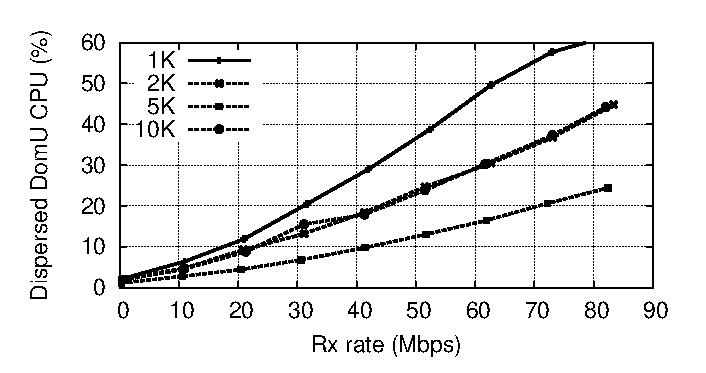
\includegraphics[scale=0.75]{jss-figures/kvm-aff-benchmark/domu-disp-cpu-for-rx-diff-file-sizes-notsoboth-kvm.eps}} ~~
	\subfloat[Colocated Guest VM CPU utilization for Rx]{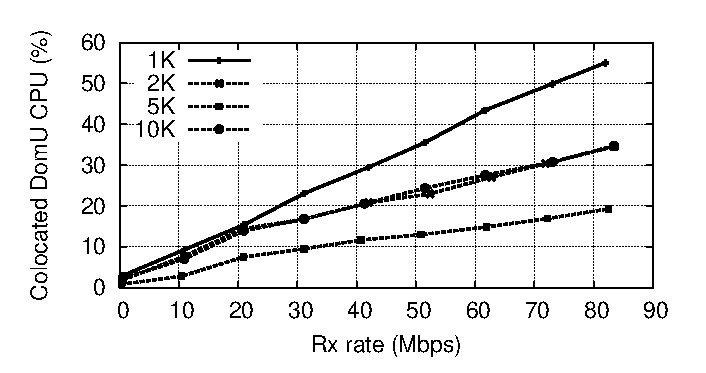
\includegraphics[scale=0.75]{jss-figures/kvm-aff-benchmark/domu-colo-cpu-for-rx-diff-file-sizes-notsoboth-kvm.eps}}
	\caption{CPU utilization for mutable receive traffic with different segment sizes (in KVM setup).}
	\label{fig:kvmdomurx-chunks}
\end{figure*}

\begin{figure*}[t]%
	\centering
	\subfloat[Dispersed Guest VM CPU utilization for Tx]{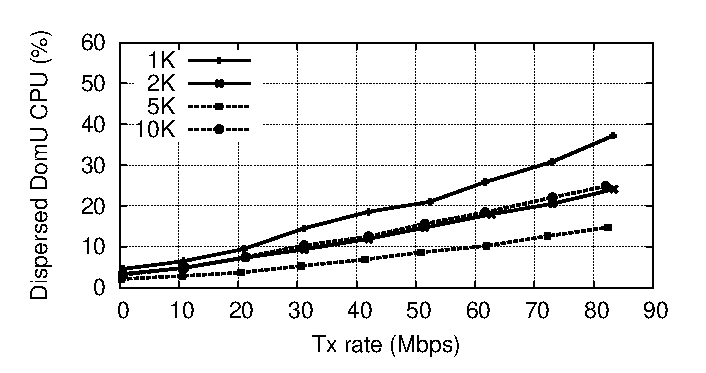
\includegraphics[scale=0.75]{jss-figures/kvm-aff-benchmark/domu-disp-cpu-for-tx-diff-file-sizes-notsoboth-kvm.eps}} ~~
	\subfloat[Colocated Guest VM CPU utilization for Tx]{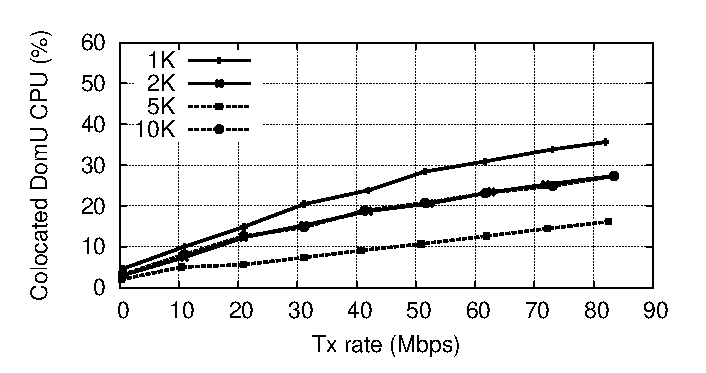
\includegraphics[scale=0.75]{jss-figures/kvm-aff-benchmark/domu-colo-cpu-for-tx-diff-file-sizes-notsoboth-kvm.eps}}
	\caption{CPU utilization for mutable transmit traffic with different segment sizes (in KVM setup).}
	\label{fig:kvmdomutx-chunks}
\end{figure*}

\paragraph{II. Impact of mutable network traffic in KVM.}
\label{sec:2ndchap-kvm-benchmark}
Similar to the benchmarking for Xen presented above, we performed
an empirical study of colocation effects in KVM as well.
As mentioned earlier, KVM does not have the concept of a privileged
domain to arbitrate I/O access amongst the VMs. Instead, each VM
is similar to a process and invokes the QEMU\index{QEMU} emulator to
access the
I/O devices. Thus, the overhead related to I/O processing (and the
resulting effects due to dispersed and colocated network
communication) would be reflected in the VM (DomU) CPU usage itself.
Fig.~\ref{fig:kvmdomurx-chunks} and Fig.~\ref{fig:kvmdomutx-chunks}
show CPU utilization
of the DomUs in dispersed and colocated scenarios in KVM\index{KVM}
setup. The experiment setting is such that VM1 requests varying
network rates in the range 10 to 80Mbps for
% (when VM1 requests, it plays
% the receiving domain role and VM2 is the transmitting domain) 
each segment size while VM2 requests a fixed rate of 10Mbps.
Thus, though both VMs are transmitting and
receiving data, the variations in network rate at a given
segment size setting are caused only by VM1's request-rate.

Fig.~\ref{fig:kvmdomurx-chunks} shows that when receive traffic
at VM1 is 80Mbps for a segment size of 10KB, DomU CPU usage is
44\% absolute CPU in dispersed case and drops to 35\% in colocated case
whereas for segment size of 1KB, CPU usage drops from 62\% in
dispersed case to 55\% in colocated case. Similarly,
Fig.~\ref{fig:kvmdomutx-chunks}
shows CPU usage plots for VM2 transmitting 80Mbps using
%the transmitting domain for 
various
segment sizes. Thus, we observe that CPU usage of transmitting
and receiving DomUs change between colocated \& dispersed scenarios.
Additionally, we also observe that CPU utilization
is approximately linear with respect to network utilization in
above experiments.


%%%%%%%%%%%%%%%%%%%%%%%%% nonaff-rx
\begin{table}
\caption{Percentage CPU usage for \textit{immutable} Rx.}
\centering
% \noindent\makebox[\textwidth]{% 
\begin{tabular}{|c|c|c|} \hline
\textbf{Immutable} & \multicolumn{2}{|c|}{\textbf{Percentage CPU utilization}} \\ \cline{2-3} \cline{2-3}
\textbf{Receive} & \textbf{Dispersed case} & \textbf{Colocated case} \\
(Mbps) & $VM_1,VM_2, \sum Dom0_i$ & $VM_1,VM_2,Dom0$ \\ \hline
% $<$20, 10$>$ & 3, 2, 12 & 3, 2, ~8 \\ \hline
% $<$20, 30$>$ & 4, 5, 14 & 3, 5, 11 \\ \hline
$<$20, 50$>$ & 4, 7, 18 & 4, 7, 14 \\ \hline
$<$20, 70$>$ & 4, 9, 21 & 4, 9, 17 \\ \hline
$<$40, 10$>$ & 6, 2, 15 & 6, 2, 11 \\ \hline
$<$40, 30$>$ & 7, 5, 18 & 7, 5, 15 \\ \hline
$<$40, 50$>$ & 7, 7, 21 & 7, 7, 18 \\ \hline
$<$60, 10$>$ & 8, 2, 18 & 8, 2, 14 \\ \hline
% $<$60, 30$>$ & 8, 5, 21 & 8, 5, 18 \\ \hline
\end{tabular}
% }
%\caption{Non-affine receive benchmarking results for colocated provisioning}
\label{nonaff-rx-benchmark}
%\vspace{-0.3in}
\end{table}

\paragraph{III. Other workloads.}
Table~\ref{nonaff-rx-benchmark} shows colocated benchmarking
results for immutable \textit{receive} traffic\textemdash{}VMs receiving 
network packets from ``dispersed'' (i.e. hosted on different PMs) transmitters. 
The table shows CPU usage of VMs in
dispersed and colocated cases for Dom0 and DomU.
The left most column shows tuples of the form $<x,y>$ where
$x$ is the the receive rate at VM1 and $y$ is the receive
rate at VM2. The second column shows the CPU utilization of 
VM1, VM2 and the summation of the CPU utilization of the two 
Dom0 instances in dispersed scenario. The third column shows
the CPU utilization of VM1, VM2 and the single Dom0 instance
in the colocated scenario.
Observe that
DomU CPU utilization stay similar in both dispersed \& colocated
cases.
The colocated Dom0
CPU utilization is consistently (4\%) less than 
the summation of the Dom0 utilization
levels in the dispersed case.

Similar observation was made for other workloads\textemdash{}immutable
transmit traffic, CPU workloads, disk read and disk write workloads. 
The Dom0 utilization of 4\% is the same as its utilization
under idle load, hence the above observation implies that for all
other workloads except mutable traffic, colocation results in saving
the CPU overhead related to an extra Dom0 instance.
%More detailed results can be found in the related technical report 
%at \cite{affine-modeling-tech-report}.

\paragraph{IV. Summary of benchmarking}
From the benchmarking phase, we have following take-aways,
\begin{itemize}
  \item When the nature of mutable network traffic changes between intra-PM
				  and inter-PM, there
				  is a change in guest VM CPU utilization in both Xen
				  and KVM environments. 
				  %, and this change is dependent on not only the
%				  network rate but also the application segment size.
  \item In case of Xen Dom0, change in nature of network-affinity results
				  in significant change (up to 25\% absolute CPU) when comparing
				  colocated Dom0 against the summation of dispersed Dom0 utilization.
  \item With increase in network utilization, 
	  the increase in CPU utilization is linear
			 in both Xen and KVM environments.
	\item For all workloads, other than mutable network traffic, colocation results
		in similar DomU CPU usages in both colocated and dispersed cases.
	\item For all workloads, other than mutable network traffic, the summation of CPU 
		usage of the two Dom0 instances in dispersed case differs from the 
		colocated CPU usage by a constant amount (say 4\% absolute CPU). 
\end{itemize}
		  
\textit{Based on the results of benchmarking, we
			  conclude that the relation between increase in network utilization
		  and CPU utilization is linear for both Xen and KVM environments.}
		  \footnote{These results are applicable only when both the network
			  and CPU resources have spare capacity, e.g., if CPU utilization is
			  already close to 100\%, increasing the network rate is either not
			  possible or results in no corresponding change in CPU utilization.
			  All further observations, modeling and inferences are based on this
		  premise.} As a result, both the ``total'' as well as 
		  the ``differences'' in CPU utilization can be
		  captured using linear estimation models.


%\paragraph{III. Summary of Xen benchmarking with colocation.}
%From the above set of benchmarking experiments, 
%we conclude that 
%For mutable network traffic, there is
%marginal reduction in DomU CPU utilization after colocation and
%significant savings (up to 25\%) in Dom0 CPU utilization.

%clipped 10feb
\subsection{Feasibility of Generic models}
In order to build a model that can be generically used to
predict CPU utilization of DomUs, 
even though it is trained on only one or couple of VMs,
it is necessary that VMs behave similarly under
similar loading conditions. 
For example, suppose a CPU load of
$x\%$ is requested, but creates $x+5\%$ CPU load on one VM.
%As mentioned before, this accuracy is enough for our benchmark
%profiling, however, 
It is essential that the same load when
requested on another homogeneous VM, results in similar
resource utilization levels. 
% This is a very basic expectation
% % and we present some sample results to demonstrate that this
% % does indeed hold. 
Thus, we are interested in verifying the 
following two hypotheses\textemdash{}(i) Given similar 
configurations, CPU utilization for similar load levels on 
different VMs match up, (ii) Given similar platforms, CPU 
utilization for similar loads on same VM but different PMs match up.
 
To this end, we performed several repeatable experiments 
on two VMs that were placed in a dispersed manner and compared whether 
similar loads result in similar CPU utilization levels on both VMs
and their Dom0s. We performed such experiments for all load 
types\textemdash{}CPU intensive, mutable traffic, immutable traffic
and disk-intensive\textemdash{}and as expected, we observed that both the
above hypotheses about CPU utilization on different VMs 
and PMs held true.
\\
\\
In this section, we established the basic benchmarking results that
will be applied to develop a generic CPU estimation model. By generic,
we imply that a single model would be able to estimate CPU utilization
for any given application, without requiring re-training on the specific
application itself.
In the next section, we present our approach to develop the generic
model and use it to estimate the CPU usage when a pair
of VMs are colocated or dispersed.


\label{sec:arescue-benchmark}

%\section{Our Approach: A-RESCUE}
\section{Linear regression modeling for absolute CPU requirement estimation}


This section presents the core idea of our model generation and usage methodology.
%As mentioned earlier, our interest is to build a model that can capture the
%relationship between the resource utilization profiles and resultant CPU
%utilization when a pair of VMs transition from being dispersed to colocated,
%or vice versa.
We run a set of benchmarks, also referred to as micro-benchmarks, in both 
scenarios\textemdash{}dispersed and colocated\textemdash{}which exercise the utilization 
levels of VMs along different
axes\textemdash{}CPU, mutable and immutable network traffic, disk read and
write operations.


 \begin{table}
 \caption{Metrics considered per load type on each DomU (for predicting total CPU).}
%  \hspace{-0.2in}
 \begin{center}
 \begin{tabular}{|l|c|c|l|} \hline
  \bf{Disk} & \bf{Mutable} & \bf{Immutable} & \bf{CPU} \\ 
 & \bf{network} & \bf{network} & \\
  & \bf{traffic} & \bf{traffic} & \\ \hline
  Read (bytes/s) & Rx (Kbps) & Rx (Kbps) & User (\%) \\
  Write (bytes/s) & Tx (Kbps) & Tx (Kbps) & System (\%) \\
  Read (blocks/s) &  &  & Iowait (\%) \\
  Write (blocks/s) & &  & \\ \hline
 % Write blocks/sec & (NA) Tx Kbps & (A) Tx Kbps & System CPU\% \\
 %  &  &  & Iowait \\ \hline
 \end{tabular}
 \label{metrics-table}
 \end{center}
 \end{table}

\underline{Colocation and Dispersion models}: We wish to 
develop pair-wise CPU estimation models
that can predict total CPU requirement in target scenario
based on source scenario's resource usages.
Specifically, using resource usage measurements in
dispersed scenario, the ``colocation''
model predicts CPU utilization for VMs in the colocated scenario,
while the ``dispersion''
model uses resource usage measurements in the colocated scenario and 
predicts CPU utilization of VMs in the dispersed scenario.

Our benchmarking revealed that only the mutable network usage
causes change in CPU usage, upon change in VM placement.
Hence, we employ \underline{two approaches of prediction}:-
(i)~Predict \textit{total} CPU requirement based on multiple
resource usage profiles\textemdash{}CPU, disk and network,
(ii)~Predict \textit{differential} CPU requirement based only on
mutable network traffic metrics\textemdash{}later, take summation
of prediction with the source scenario's CPU usage to estimate
the total CPU requirement.
Next, we explain both approaches in detail.

\subsection{Approach 1: Prediction of total CPU requirement}

\paragraph{Core Idea: } Using the profiling data from 
execution of micro-benchmarks and strengthened
by our conclusions in Section~\ref{sec:arescue-benchmark}, we 
believe that a generic linear model to estimate 
\textit{total} (dispersed or colocated) CPU resource usage
is realizable. 
The total CPU requirement of a virtual machine accounts for all its
activities, including usage of all other resources. Hence, the model
for predicting total CPU requirement has all resource metrics as its
parameters: (i)~$4$ metrics for mutable and
immutable transmit and receive network rates (in Kbps),
(ii)~$3$ CPU metrics of \texttt{iowait}, \texttt{system}
and \texttt{user} CPU (in \%), and
(iii)~$4$ metrics among disk read/write rates in
blocks/second and bytes/second. These metrics are
tabulated in Table~\ref{metrics-table}.
Since the correlation of all resource usages to CPU usage is linear, we employ
linear regression methods to build the models for CPU estimation.

\paragraph{Micro-benchmark Profiling: } The idea is to capture 
behaviour of resource usage in all possible conditions
for both dispersed and colocated scenarios. So, the micro-benchmarks
should span the full range of resource utilization levels. 
The workload micro-benchmarks are generated using the workload
generation procedures described in Section~\ref{sec:arescue-workloadgen}.
For CPU micro-benchmarking, we split the CPU load on each VM
into $nine$ different intensities
ranging from $10\%$ to $90\%$. 
For network loads, we vary the load on each VM by steps 
of 10 Mbps, from 10 to 90 Mbps.
For disk read and write
micro-benchmarking, we vary the disk read/write rate from 
0 to 1280 blocks/second on each VM.

% Next, we describe briefly
% the approach adopted to ensure that we representatively
% cover the full range of resource utilization levels.

%For our profiling step, we use a generic client-server setup (described
%in more detail in Section~\ref{fig:setup}), wherein a \textit{client}
%(the controller machine) remotely connects to 
%the \textit{servers} (each PM or Dom0,
%and VM or DomU). % where workload is to be generated. 
%The workload generation
%tool resides on each such ``server'' and complies with the 
%load generation
%requests received from the ``client'' machine.
% 
% \textbf{SSS:Write up about micro-benchmarks. Also, mention
% the exponential number of cases to consider for combinational loads, and hence
% the randomized choice of combinational load cases.}

%clipped 10 feb
% \begin{itemize}
% \item \textbf{CPU micro-benchmark.}
% For CPU micro-benchmarking, we split the CPU load 
% into $nine$ different intensities
% ranging from $10\%$ to $90\%$. At each of the two VMs, 
% we vary the CPU load from $10\%$ to $90\%$, thus 
% resulting in $9 \times 9 = 81$ CPU workload
% combinations, as input for the modeling process.
% 
% \item \textbf{Network micro-benchmark.} 
% For network loads, we assume the maximum available capacity 
% to be $100Mbps$ and vary the load on each VM by steps 
% of $10Mbps$, from $10$ to $90 Mbps$.
% 
% \item \textbf{Disk read \& write micro-benchmarks.}
% For disk read and write
% micro-benchmarking, we vary the disk read/write rate from 
% 0 - 1280 blocks/second on each VM.
% For all files read and written, the block size is retained as $4 KB$.
% \end{itemize}


The set of inputs to train/build the models also includes 
combination workload benchmarks, which have CPU, network and disk
loads executed simultaneously, with different combinations of 
utilization levels.
However, to conduct exhaustive experiments that cover the
entire combination input set is not possible, since there is an
exponential number of cases in the input space of combinational load.
Thus, we adopted a workaround of choosing a set of random input 
workload levels. 
For each combination benchmark, we sample a target utilization level, for 
each workload type, from a pre-defined range\textemdash{}CPU utilization from $10\%$ to 
$90\%$, network rate from 10 Mbps to 90 Mbps and disk read/write rate
of $0$ - $1280$ blocks/second. Each sample for a workload type is chosen
uniformly at random. 
This is intended to keep the sample points
uniformly distributed throughout the available sample space. 

Overall, for the model building, we used 956 sample points in total, consisting
of 200 points for CPU workload, 96 points for mutable network usage, 182 points
for immutable network usage, 162 points for disk read workload, 158 points for disk write 
workload and 158 combinational workloads.
% Thus, a combinational load input to a single VM would
% be a 6-tuple of the form,
% $<$\textit{c}$\%$, $a$ Mbps, $nrx$ Mbps, $ntx$ Mbps, $r$, \textit{w}$>$ \\ 
% where,
% $c$ is a random number in [1-100] for generating $c$\% CPU load,
% $a$ is a random number in [1-90] for generating $a~Mbps$ affine network
% receive traffic (correspondingly $a~Mbps$ transmit
% traffic at the other VM),
% $nrx$ is similarly random in [1-90] for generating non-affine network
% transmit traffic, 
% $ntx$ is random in [1-90] for generating non-affine network
% transmit traffic, 
% $r$ and $w$ are randomly chosen file read/write
% rates between 0 - 1280 blocks/second. Note that given a pair of VMs,
% the affine network traffic transmitted by one VM is the affine network
% traffic received by the other.



% \paragraph{Profiling Resource Usage:}
% We use the same setup as shown in Section~\ref{initial-benchmarking} (refer Fig.~\ref{f14})
% for the load generation and logging, described in this section. 

% \begin{table*}[t]
% \begin{center}
% \begin{tabular}{|l|l|l|l|} \hline
% Disk & Non-affine(NA) network & Affine(A) network & CPU \\ \hline
% Read req/sec & (NA) Rx Kbps & (A) Rx Kbps & CPU\% \\
% Write req/sec & (NA) Tx Kbps & (A) Tx Kbps & \\ \hline
% \end{tabular}
% \caption{Tabulation of metrics for black-box approach considered per load type on each DomU.}
% \label{blackbox-metrics-table}
% \end{center}
% \end{table*}

\paragraph{Multi-Linear Regression Modeling: }
Since the correlation of various resource usage metrics 
in the dispersed (colocated)
case to CPU utilization level in the colocated (dispersed) 
case emerged as approximately linear, we employ 
linear regression methods to build the models for CPU estimation.
Using values from the collected profiling data,
%a set of equations which represent the colocated CPU usage
the colocated CPU usage is represented as 
a linear function of the individually profiled resource metrics
in the corresponding dispersed scenario (i.e. dispersed scenario
stressed with the same workload),
and similarly dispersed CPU usage is represented as a linear function of 
the colocated resource usage metrics.
% Each such equation will be of the form as shown in Eqn. (\ref{mlr-eqn})
The relation between estimated CPU and resource parameters is shown
in Eqn. (\ref{mlr-eqn}).
\begin{equation}
\mbox{CPU}^{i}_{estimated} = C_{0} + C_{1} \times M^{i}_{1} + C_{2} \times M^{i}_{2} + ... + C_{m} \times M^{i}_{m}
\label{mlr-eqn}
\end{equation}
where, $i$ is an iterator over each experiment or sample point
to be considered in the modeling, $m$ is
the number of parameters being considered, $M^{i}_{j}$ is
the value of parameter $M_{j}$ collected in the benchmark experiment number
$i$, and $\mbox{CPU}^{i}_{estimated}$ is the CPU usage 
either after dispersion or after colocation of VMs.
% The models that estimate the colocated CPU usage are referred 
% to as \textit{forward} models while 
% those that estimate the dispersed CPU utilization from the 
% colocated resource usage metrics are referred to as 
% \textit{reverse} models.
% In a \textit{forward} model, Dom0 %and DomU CPU usages
% CPU savings
% with colocated provisioning are predicted based on
% resource usages of VMs in the dispersed placements.
% In case of a
% black-box model (both forward and reverse), $m = 11$, and 
%The parameters considered per VM are, (i) $4$ metrics for mutable and 
%immutable transmit and receive network rates (in Kbps), 
%(ii) $3$ CPU metrics of \texttt{iowait}, \texttt{system} 
%and \texttt{user} CPU (in \%), and 
%(iii) $4$ metrics among disk read/write rates in 
%blocks/second and bytes/second. 
There are $11$ metrics in all to be considered, as discussed 
earlier in Table~\ref{metrics-table}. 
Both the colocation and dispersion DomU models have all these $11$ parameters.
The Dom0 \textit{colocation} model is built
with the metrics of both DomUs, and hence has $22$ parameters. 
The Dom0 \textit{dispersion} model 
depends on only one DomU's metrics at a time, and hence has only $11$
parameters.
% just like the DomU model. 
This is because the dispersed Dom0's CPU usage intuitively
depends on the resource usage of only its own hosted DomU and 
not on the other DomU of the VM pair.

\subsection{Approach 2: Prediction of differential CPU requirement}
\paragraph{Core idea: }
The difference in CPU usage upon transition between
colocated and dispersed placements of a VM pair, depends only on the mutable
network affinity between them. Hence, the idea here is to predict only
the difference, and sum it with the original scenario's CPU usage, to
obtain the total CPU requirement.
Note that differential Dom0 CPU is the difference in CPU 
usage between that incurred for the single (colocated) Dom0 and
the summation of both (dispersed) Dom0.
The model parameters are bit-rates (in Kbps) and packet-rates (in packets 
per second) for both transmission (Tx) and reception (Rx), thus four parameters
in all: (i) Rx Kbps, (ii) Rx pkts/s, (iii) Tx Kbps, and (iv) Tx pkts/s. 

\paragraph{Modeling of differential CPU utilization: }
Since we predict only the difference in CPU usage, the total
CPU requirement of the migrating VM on the target can be computed
as the sum of the predicted value and the observed CPU usage on
the source PM. Formally, Eqn. (\ref{cpu-diff-eqn}) captures the
general notion of change in CPU usage ($\Delta\mbox{CPU}$)
while transitioning between colocated and dispersed scenarios.
\begin{equation}
	% \hspace{-0.3in}
	\Delta\mbox{CPU} = \mbox{CPU}^{scenario1} - \mbox{CPU}^{scenario2}
	\label{cpu-diff-eqn}
\end{equation}
where, scenario$\{1|2\}$ = $\{colocated|dispersed\}$.
In case of \textbf{Dom0's CPU usage}, colocated Dom0 CPU usage is incurred
for hosting both VMs whereas dispersed Dom0 usage levels are
on behalf of a single VM each. During transition from dispersed
(\textit{disp} in short) to colocated (\textit{colo} in short),
the change in Dom0 CPU is defined as the difference in CPU usage
between that incurred for the single (colocated) Dom0 and the
summation of both (dispersed) Dom0, as illustrated in
Eqn. (\ref{dom0-diff-eqn-fwd}).
%\hspace{-0.2in}
\begin{equation}
	% \hspace{-0.3in} \mbox{CPU}^{dom0}_{diff} = \mbox{CPU}^{{dom0}_{1}}_{dispersed} + \mbox{CPU}^{{dom0}_{2}}_{dispersed} - \mbox{CPU}^{dom0}_{colocated}
	% \hspace{-0.3in} 
	%\delta\mbox{Dom0CPU}^{colo} = \mbox{Dom0CPU}^{colo} - \displaystyle\sum\limits_{i=1,2}\mbox{Dom0CPU}^{disp}
	\Delta\mbox{CPU}^{colo}_{Dom0} = \mbox{CPU}^{colo}_{Dom0} - \displaystyle\sum\limits_{i=1,2}\mbox{CPU}^{disp}_{Dom0}
	\label{dom0-diff-eqn-fwd}
\end{equation}
Similarly, during transition from colocated to dispersed, change in
CPU usage for each Dom0 instance is,
\begin{equation}
	% \hspace{-0.2in} 
	\Delta\mbox{CPU}^{disp}_{Dom0} = \mbox{CPU}^{disp}_{Dom0} - \frac{\mbox{CPU}^{colo}_{Dom0}}{2} %\frac{{CPU}^{dom0}_{colocated}}{2} 
	\label{dom0-diff-eqn-rev}
\end{equation}
% where i = 1,2.
Here we use %$\frac{{CPU}^{dom0}_{colocated}}{2}$ 
$\mbox{CPU}^{colo}_{Dom0}$/2
% as an approximation of CPU usage incurred
% for a single VM within the colocated scenario. Intuitively, the Dom0
% CPU usage incurred per VM in a colocated setting is different than
% that incurred in a dispersed setting, when intra-PM traffic is involved.
% This is % in Eqn. (\ref{dom0-diff-eqn-rev}) 
since colocated Dom0 CPU usage
is incurred on behalf of both VMs whereas we wish to predict
dispersed Dom0 CPU usage incurred on behalf of only a single VM each.
So, we use $\mbox{CPU}^{colo}_{Dom0}$/2 as an approximation of CPU usage
incurred for a single VM within the colocated scenario.
% so that the difference between Dom0
% usage on behalf of each VM in colocated and dispersed cases can be computed.
In case of \textbf{DomU's CPU usage}, we define change
in CPU as shown in Eqn. (\ref{domu-diff-eqn}).
\begin{equation}
	\Delta\mbox{CPU}_{DomU} = \mbox{CPU}^{disp}_{DomU} - \mbox{CPU}^{colo}_{DomU}
	\label{domu-diff-eqn}
\end{equation}
Based on Eqn. (\ref{domu-diff-eqn}), the difference needs to
be added to or subtracted from the observed CPU usage depending upon
whether the VM's migration results in dispersion or colocation, respectively. 
Thus, DomU's
colocation and dispersion models are one and the same, since the
\textit{magnitude} of the difference in CPU usage is the same in both
directions.

Using values from the collected profiling data,
%a set of equations which represent the colocated CPU usage
difference in CPU usage is represented as a linear function of the
individually profiled network usage metrics in dispersed
scenario (i.e. dispersed scenario stressed with the same workload).
The relation between estimated CPU and resource parameters is the
same as shown earlier in Eqn.~\ref{mlr-eqn}, except that
the value being estimated is the difference in CPU usage
and not the total.
In case of DomU model, the CPU usage estimate is expectedly a
function of its own network usage rates and uses all these four
metrics in its model. Similarly, in the case of Dom0 colocation model,
colocated Dom0 CPU usage accounts for both the colocated DomUs
and hence should intuitively depend on four metrics each of
both the DomUs, i.e. eight metrics in total. However, given a VM pair
with only mutual network communication, the received traffic by one
VM is the transmitted
traffic by the other, hence metrics of one VM are in fact
duplicates of metrics of the other, albeit in a different
order. We discard the redundant columns, therefore even Dom0
model has only four parameters. Thus, each model can be represented as
\begin{equation}
	% \mbox{CPU}_{est} = C_{0} + C_{1} \times Aff^{Rx}_{MBps} + C_{2} \times Aff^{Tx}_{MBps} + Aff^{Rx}_{pps} + Aff^{Tx}_{pps}
	% \hspace{-0.3in} \mbox{CPU}_{est} = C_{0} + C_{1} Aff^{R}_{K} + C_{2} Aff^{T}_{K} + C_{3} Aff^{R}_{P} + C_{4} Aff^{T}_{P}
	%\begin{split}
	\hspace{-0.3in} \Delta\mbox{CPU}_{est} = C_{0} + C_{1} \mbox{MutRx}_{Kbps} + C_{2} \mbox{MutRx}_{p/s} \\ 
	+ C_{3} \mbox{MutTx}_{Kbps}  + C_{4} \mbox{MutTx}_{p/s}
	%\end{split}
	\label{mlr-eqn-2}
\end{equation}
 where, ``Mut'' represents mutable network traffic,
  superscripts Rx \& Tx represent receive \& transmit, and
  subscript p/s represents the units packets/second.
\\
\\
To solve for the $m+1$ coefficients $C_{k}$, a stepwise linear
regression approach can help to select the ``best'' set of parameters.
%, in a stepwise manner.
% that would result in the most optimal prediction for the given learning dataset. 
% Thus, a model is learnt based only on these selected set of metrics. 
The stepwise approach ensures that only significant parameters that influence 
the predicted value are part of the model~\cite{applied-regression-analysis}.
For our implementation, we use the
% LARS~\cite{lars} package %present in Python~\cite{python} 
Robustbase package~\cite{robustbase}, part of the R statistical computing
environment, for robust and stepwise linear regression.
The linear regression solver, takes as input $M^{i}_{j}$ values for the 
various workloads and outputs values of $C_{k}$ that 
best predict CPU utilization. The set of coefficients thus
derived is the model that describes the relation between the $k$ parameters
and the total or differential CPU usage.

\subsection{Applying the pair-wise models to multi-VM scenarios}
\label{sec:multi-vm}
In order to apply the pair-wise models to situations with multiple
VMs hosting different applications
that may have different number of communicating tiers, the
first step needed is to consider that in a multi-VM scenario,
a single VM migration step
can result in not only dispersion w.r.t one (or a few) VM(s), but
also in colocation w.r.t other VM(s).
%To be more specific, the models that we have constructed so far
%apply to a single pair of VMs at a time i.e., in a single VM
%migration step, either two dispersed
%VMs can get colocated or two colocated VMs can get dispersed.
%In order to apply this CPU usage model to a real multi-VM 
%scenario, we need to be able to predict the CPU utilization 
%even in a combined scenario, wherein 
Fig.~\ref{fig:forward-plus-reverse} illustrates the case where
a single VM is being dispersed from one VM and colocated with another.
%Note that the terms DomU and VM are used interchangeably
%in this description and figure. 
Suppose $VM1$, $VM2$ and $VM3$ host different tiers of a 3-tier application.
As can be seen, one VM migration can result in that VM ($VM2$ in
Fig.~\ref{fig:forward-plus-reverse}) being dispersed from one VM ($VM1$)
on the source PM and being colocated with another VM ($VM3$) on
the target PM.

%Further, a VM that is communicating with multiple
%colocated VMs would get dispersed from all of them due to a single
%migration step. 
In the general multi-VM scenario, any particular VM (say $VM_{x}$)
may have multiple communicating neighbors, each of them belonging to
exactly one of three sets, (i) \textit{affinity-at-source}
(ii) \textit{affinity-at-target}, and (iii) \textit{affinity-at-other}.
Migration of $VM_{x}$ will cause it to become dispersed from
its \textit{affinity-at-source} set and colocated with its
\textit{affinity-at-target} set.
We refer to this dual step of being dispersed from
\textit{affinity-at-source} set and being colocated with
\textit{affinity-at-target} set, as a \textit{combined transition}.
In this case, the CPU utilization of all VMs in the
\textit{affinity-at-source} \& \textit{affinity-at-target} sets and
the migrating VM itself are expected to change.
In fact, the \textit{colocation}
and the \textit{dispersion} transitions can be viewed as
special cases of the \textit{combined} transition, starring only 
two VMs, with the dispersion transition being the case where 
dispersion set on source PM is empty while the dispersion transition 
is the case with an empty set on target PM.
Our aim is to predict the resource usage of all affected VMs and PMs.

\begin{figure}[t]
	\centering
	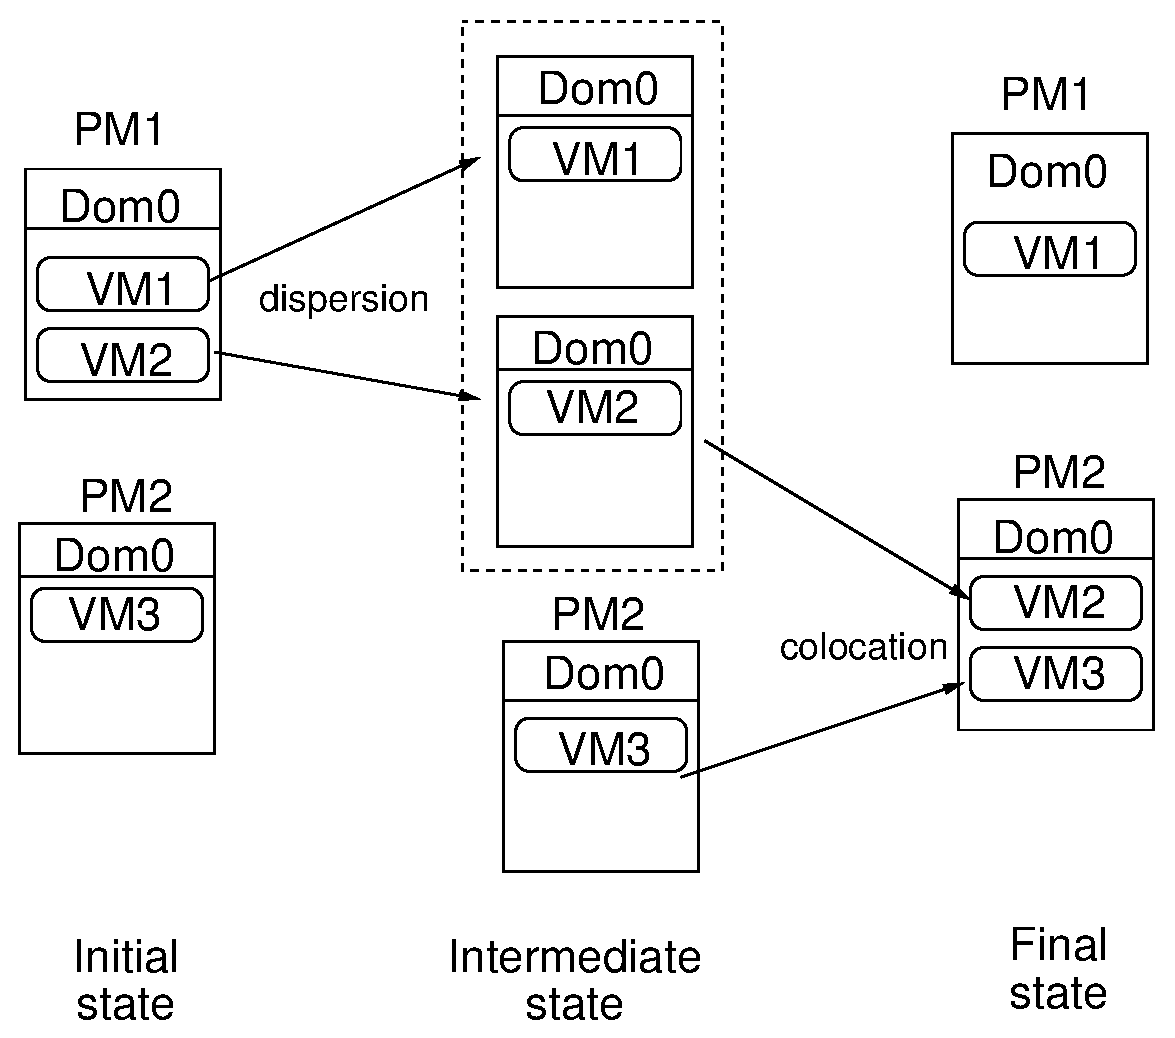
\includegraphics[scale=0.45]{jss-figures/new-forward-plus-rev.eps}
	\caption{Combined transition for $VM2$}
	\label{fig:forward-plus-reverse}
\end{figure}
% Our aim is to predict the CPU utilization when $VM2$'s migration
% causes a change in placement from \textit{Configuration1} to \textit{Configuration2}
% or vice versa. 

Consider the combined transition illustrated in Fig.~\ref{fig:forward-plus-reverse}.
It is straight-forward
to apply the DomU \textit{colocation} and \textit{dispersion} models to
$VM1$ and $VM3$ to predict their resultant CPU usages. Similarly, $PM1$'s
Dom0 CPU usage can also be predicted by applying Dom0 dispersion model.
However, prediction of $VM2$'s and $PM2$'s resultant CPU usage after this
combined transition needs a multi-phase prediction methodology.
The basic idea is to first apply the \textit{dispersion model} to the
measured metrics corresponding to network-affinity level between $VM2$
to/fro the \textit{affinity-at-source} set, and then use this
intermediate estimate
%This is an intermediate estimate and is used 
to make final prediction based upon network-affinity level
between $VM2$ to/fro the \textit{affinity-at-target} set. Incidentally,
VMs in the \textit{affinity-at-other} set do not affect $VM2$'s CPU
requirement because the nature of network-affinity
between them and $VM2$ is \textit{immutable} w.r.t its migration.
\\
\\
In this section, we described our model-building process and described
the synthetic training datasets used to learn this model.
We also described the process of applying the pair-wise prediction
models to multi-VM scenarios.
Though the models are built with synthetic datasets in which
TCP data-rates are generated by manipulating the application level
segment size and the periodicity of transmission, the application
scenarios for the models are not expected to have such controlled
behaviour. In particular, though the applications are
expected to use TCP for communication, the application-level
segment sizes and the inter-request times (also called think-times)
would be significantly more random. In the next section, we experimentally
evaluate the models on randomized synthetic data as well as on
benchmark application data. We also apply the model to multi-VM
scenarios and evaluate prediction effectiveness.

\label{sec:arescue-our-approach}

\section{Results and discussion}

%latest commented and above added for camera-ready
%\begin{figure}[t]
%\centering
%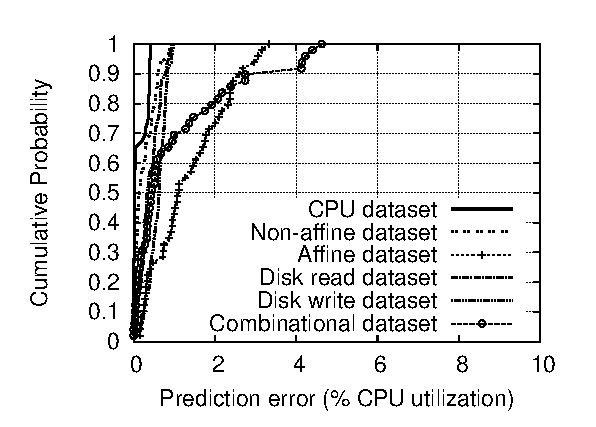
\includegraphics[scale=0.8]{synthetic-cdf-plots/dom0-forward-unseen-cdf.robust.eps}
%\caption{Prediction error CDF for \textit{colocated} Dom0 CPU estimation.}
%\label{fig:forward-unseen-cdf}
%\vspace{-0.25in}
%\end{figure}


In the previous section, we described the motivation and methodology
of developing models to predict colocated and 
dispersed CPU utilization.
After the models are built, we recompute or ``predict'' the colocated
CPU value for the training set itself, using the generated model 
coefficients. This is a sanity check to validate model correctness.
The results showed that well-fitting models 
were built, with less than 1\% to 2\% error for all workloads. However, the real test
is whether the models are able to successfully
predict the average CPU usage well, when applied to unseen data.
We present model evaluation on both synthetic data-sets and benchmark
application data in this section.


% 
% \begin{figure*}[t]
% \centering
% \noindent\makebox[\textwidth]{% 
% \begin{tabular} {cc}
% 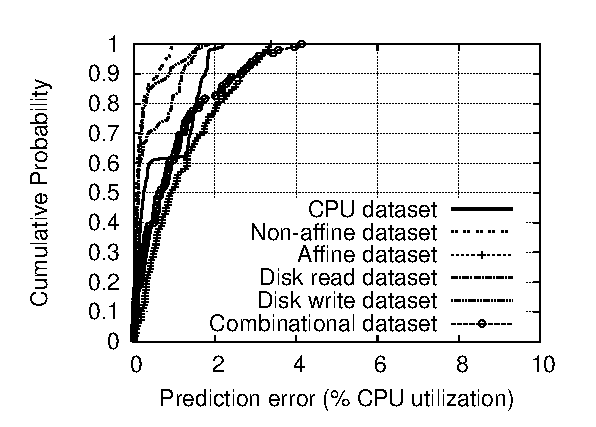
\includegraphics[scale=0.85]{synthetic-cdf-plots/domu-forward-unseen-cdf.robust.eps} & 
% 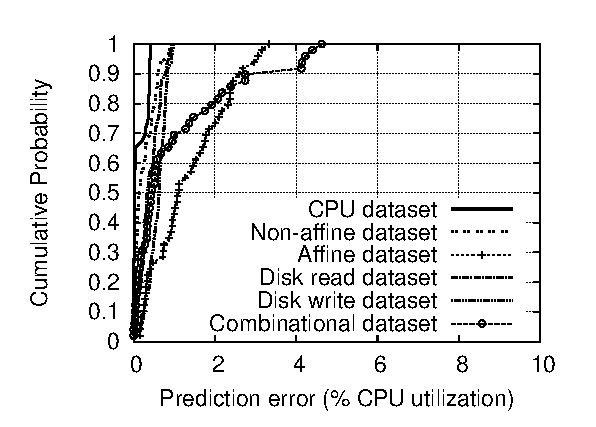
\includegraphics[scale=0.85]{synthetic-cdf-plots/dom0-forward-unseen-cdf.robust.eps} \\
% (a) DomU forward model & (b) Dom0 forward model 
% \end{tabular}
% }
% \caption{Prediction error CDF for \textit{colocated} CPU usage estimation.}
% \label{fig:reverse-unseen-cdf}
% \end{figure*}
% 
% 
% \begin{figure*}[t]
% \centering
% \noindent\makebox[\textwidth]{% 
% \begin{tabular} {cc}
% 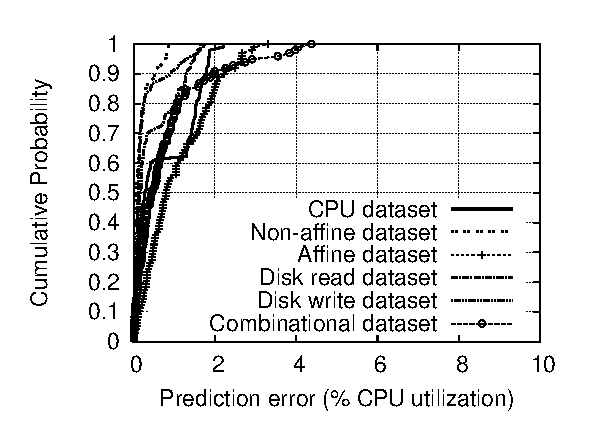
\includegraphics[scale=0.85]{synthetic-cdf-plots/domu-reverse-unseen-cdf.robust.eps} & 
% 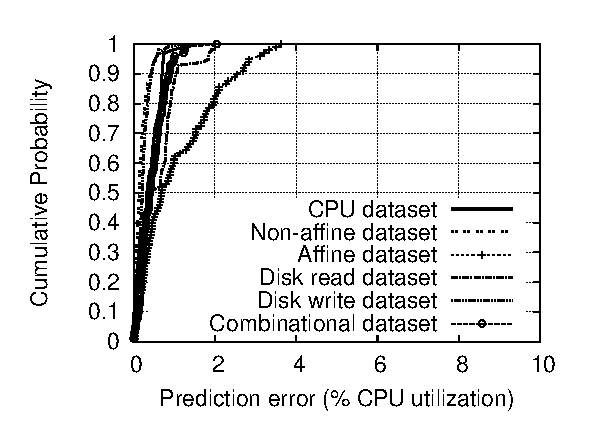
\includegraphics[scale=0.85]{synthetic-cdf-plots/dom0-reverse-unseen-cdf.robust.eps} \\
% (a) DomU reverse model & (b) Dom0 reverse model
% \end{tabular}
% }
% \caption{Prediction error CDF for \textit{dispersed} CPU usage estimation.}
% \label{fig:reverse-unseen-cdf}
% \end{figure*}

% \begin{figure*}[t]
% \centering
% \noindent\makebox[\textwidth]{% 
% \begin{tabular} {ccc}
% \includegraphics[scale=0.7]{aff-apps/rubis-co-domu1.eps} & 
% \includegraphics[scale=0.7]{aff-apps/rubis-co-domu2.eps} &
% \includegraphics[scale=0.7]{aff-apps/rubis-co-dom0.eps} \\
% (a) Web tier VM & (b) DB tier VM &  (c) Colocated Dom0 \\
% \end{tabular}
% }
% \caption{Estimating colocated CPU utilization for RUBiS using \textit{forward} models.}
% \label{fig:rubis-forward}
% \end{figure*}



% \begin{figure*}[t]
% \centering
% \noindent\makebox[\textwidth]{% 
% \begin{tabular} {rccl}
% \includegraphics[scale=0.65]{aff-apps/rubis-dis-domu1.eps} &
% \includegraphics[scale=0.65]{aff-apps/rubis-dis-domu2.eps} &
% \includegraphics[scale=0.65]{aff-apps/rubis-dis-dom01.eps} &
% \includegraphics[scale=0.65]{aff-apps/rubis-dis-dom02.eps} \\
% (a) Web tier VM & (b) DB tier VM &
% (c) Dom0 of Web tier VM & (d) Dom0 of DB tier VM \\ 
% \end{tabular}
% }
% \caption{Estimating dispersed CPU utilization for RUBiS using \textit{reverse} models.}
% \label{fig:rubis-reverse}
% \end{figure*}


% \begin{figure*}[t]
% \centering
% \noindent\makebox[\textwidth]{% 
% \begin{tabular} {cc}
% \includegraphics[scale=0.65]{aff-apps/rubis-dis-domu1.eps} &
% \includegraphics[scale=0.65]{aff-apps/rubis-dis-domu2.eps} \\
% (a) Web tier VM & (b) DB tier VM \\ 
% \includegraphics[scale=0.65]{aff-apps/rubis-dis-dom01.eps} &
% \includegraphics[scale=0.65]{aff-apps/rubis-dis-dom02.eps} \\
% (c) Dom0 of Web tier VM & (d) Dom0 of DB tier VM \\ 
% \end{tabular}
% }
% \caption{Estimating dispersed CPU utilization for RUBiS using \textit{reverse} models.}
% \label{fig:rubis-reverse}
% \end{figure*}



\subsection{Model evaluation with synthetic data-sets}
In this sub-section, we present our findings when the generated
models were applied to ``unseen'' datasets. 
By unseen, we mean that these datasets are not a part of the
input set for model creation.
The setup used for evaluation with synthetic\index{Synthetic benchmarks} 
data-sets is the same 
as the one that was presented in Section \ref{sec:arescue-setup}, 
for the benchmarking experiments.
We present the evaluation of the two approaches separately\textemdash{}predicting
total CPU usage, and predicting differential CPU usage.

\begin{figure}[t]
% \centering
\hspace{-0.2in}
\subfloat[Dom0 CPU in colocated scenario (colocation model)]{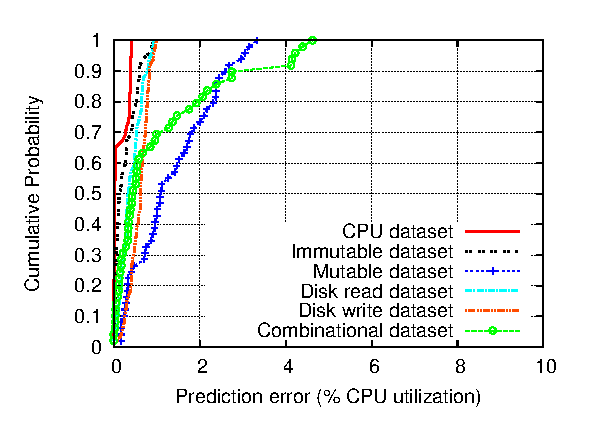
\includegraphics[scale=0.9]{arescue-figures/synthetic-cdf-plots/dom0-forward-unseen-cdf-robust.eps}}
\subfloat[Dom0 CPU in dispersed scenario (dispersion model)]{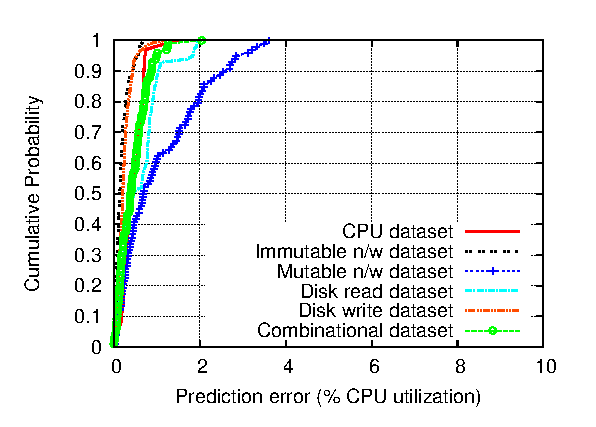
\includegraphics[scale=0.9]{arescue-figures/synthetic-cdf-plots/dom0-reverse-unseen-cdf-robust.eps}}
\caption{Prediction error CDF for Dom0 CPU estimation.}
\label{fig:dom0-unseen-cdf}
% \vspace{-0.25in}
\end{figure}

% We test the models on the following workload types \textemdash{} CPU,
% intra-PM traffic, inter-PM traffic, disk read, disk
% write and also on combinational workloads.
\underline{For models predicting total CPU usage:}
The training data input for the models was generated
by generating resource utilization at pre-defined discrete 
levels, however, the derived models
need to be applied to ``unseen'' resource usage profiles
in order to judge their adequacy. For this reason, the
CPU workload for testing consists of $100$ randomly
picked values in the range $1\%$
to $100\%$, the mutable\index{Mutable} and immutable\index{Immutable} 
Rx/Tx test workloads
are chosen randomly from the range 10 Mbps to 90 Mbps, the
disk read/write rates are randomly chosen from the range
0 to 1280 blocks/second, and the combinational workloads 
had randomly chosen values for each parameter (CPU, mutable
network traffic, immutable network traffic,
and disk) from these same ranges.

Fig. \ref{fig:dom0-unseen-cdf} plots the CDFs of error when
Dom0 \emph{colocation} and \emph{dispersion} models were applied to all the
six unseen datasets\textemdash{}cpu, mutable \& immutable network traffic, disk read,
disk write and combinational loads. It can be observed that
all the CDFs seem to stick to the left end of the graph, however,
the 90th percentile
error is around 3\% absolute CPU and maximum error is around 4\%. 
We plotted similar error
CDFs for colocated and dispersed DomU CPU estimation. In 
all cases, we found that
the 90th percentile absolute error was within 3\%. We do
not present all the CDFs here, for sake of brevity; they can
be found in the technical report at \cite{affine-modeling-tech-report}.
In case of Dom0 models\index{Dom0 model}, 
since the savings due to co-location
is significant (as concluded from the benchmarking results), an
accuracy with 3\%error might suffice for a good prediction. However, in
case of DomU models\index{DomU model}, 
the savings themselves being marginally 
lower (between 0 to 10\%), a 3\% error could imply higher 
relative error in comparison. 
% With further increase in affine 
% network rate, increased CPU utilization (and hence increased 
% savings) may still benefit from this model's accuracy.
% \begin{figure*}[t]
% \centering
% \noindent\makebox[\textwidth]{% 
% \begin{tabular} {ccc}
% \includegraphics[scale=0.65]{figures/unseen-cpu-cdf.eps} & 
% \includegraphics[scale=0.65]{figures/unseen-aff-cdf.eps} &
% \includegraphics[scale=0.65]{figures/unseen-nonaff-cdf.eps} \\
% (a) CPU dataset & (b) Affine dataset &  (c) Non-affine dataset \\
% \end{tabular}
% }
% \caption{Prediction error CDF for different datasets.}
% \label{fig:forward-unseen-cdf}
% \end{figure*}

\begin{figure}[t]
	\hspace{-0.6in}
	\centering
	\subfloat[DomU-1]{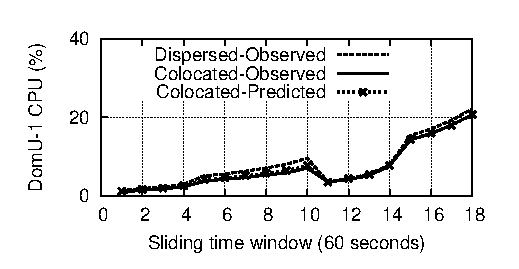
\includegraphics[scale=0.95]{jss-figures/aff-synth/synth-co-domu1.eps}}
	\subfloat[DomU-2]{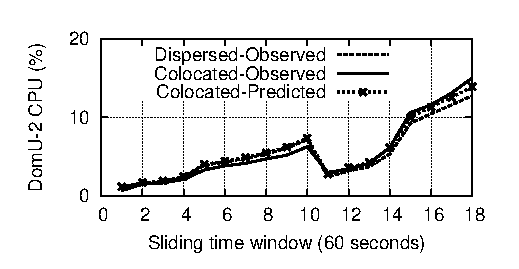
\includegraphics[scale=0.95]{jss-figures/aff-synth/synth-co-domu2.eps}} \\
	\subfloat[Colocated Dom0]{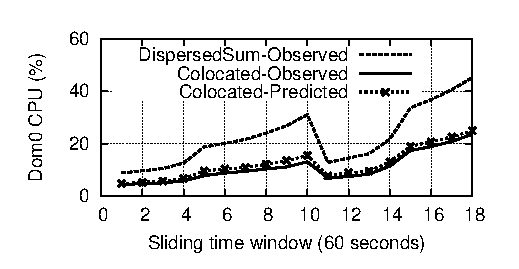
\includegraphics[scale=0.95]{jss-figures/aff-synth/synth-co-dom0.eps}}
\caption{Estimating colocated CPU utilization for synthetic data-set}% on Xen.}
\label{xensynth}
\end{figure}


\begin{figure}[t]
	\hspace{-0.6in}
	\centering
	\subfloat[Web tier VM]{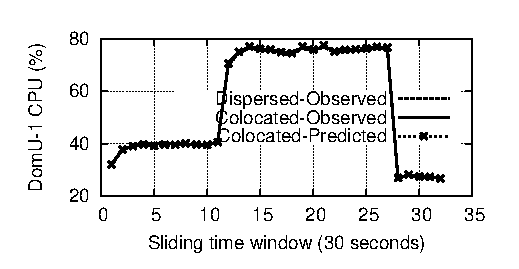
\includegraphics[scale=0.95]{jss-figures/aff-apps/rubis-3way-co-domu1.eps}}
	\subfloat[DB tier VM]{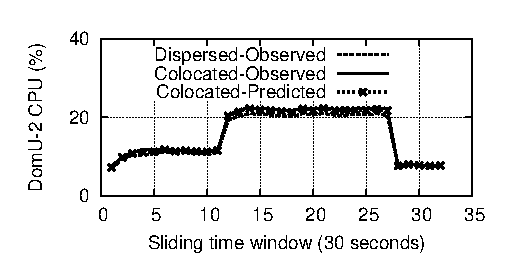
\includegraphics[scale=0.95]{jss-figures/aff-apps/rubis-3way-co-domu2.eps}}
	\\
	\subfloat[Colocated Dom0]{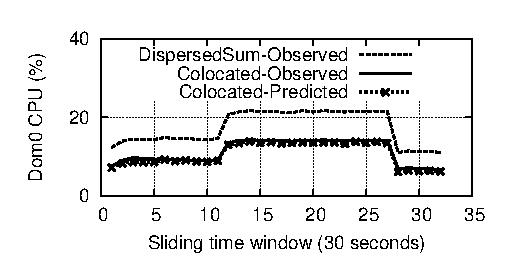
\includegraphics[scale=0.95]{jss-figures/aff-apps/rubis-3way-co-dom0.eps}}
\caption{Estimating colocated CPU utilization for RUBiS} % using \textit{forward} models.}
\label{fig:2ndchap-rubis-forward}
\end{figure}

\underline{For models predicting differential CPU usage:}
In order to generate
synthetic workload which closely emulates a real application
scenario, we spawn multiple client processes, each sleeping
for fixed intervals of time (emulating average think-time)
and generating request for transmission of varying number
of bytes or segment sizes. Thus, the artificial constraint
of each client process requesting only a single segment size
has been discarded. We generate randomly different load levels
using different number of client threads every minute, each
generating requests for different segment sizes
and monitor resource usage utilization
over a period of 18 minutes. As expected,
the resultant network traffic rates and
CPU utilization also vary.

Fig.~\ref{xensynth} shows colocated\index{Colocated}
CPU usage, predicted versus actual, for both DomUs and Dom0.
We can see that as dispersed CPU utilization
changes due to change in network usage, predicted colocated
utilization also varies similarly.
% Fig.~\ref{xensynth-cdf} shows
% the prediction error CDFs for DomU and Dom0 forward and reverse models
% when applied to this synthetic data-set. 
The maximum error in DomU prediction is within 1\% absolute
CPU usage for both DomUs (VM1 and VM2) and the maximum
error in colocated Dom0 prediction is within 2.4\% absolute CPU.
Since difference in CPU utilization for DomU is
quite low and therefore less interesting, we focus on Dom0
models here onwards.


\subsection{Model evaluation with application benchmarks}
The above evaluation with synthetic workloads demonstrated
that predicting the differential CPU usage, which considers
only the mutable network usage metrics (including both network rate
and segment size metrics) give higher accuracy predictions.
Hence, we use that approach for the rest of the evaluation
in this chapter.


%\begin{figure}[t]
%\centering
%\subfloat[Web tier VM]{\includegraphics[scale=1]{../ieeecloud2011/savefigures/aff-apps/rubis-co-domu1.eps}} 
%\subfloat[DB tier VM]{\includegraphics[scale=1]{../ieeecloud2011/savefigures/aff-apps/rubis-co-domu2.eps}}  \\
%\subfloat[Colocated Dom0]{\includegraphics[scale=1]{../ieeecloud2011/savefigures/aff-apps/rubis-co-dom0.eps}}
%\caption{Estimating colocated CPU utilization for RUBiS using \textit{colocation} models.}
%\label{fig:rubis-forward}
%% \vspace{-0.25in}
%\end{figure}


For evaluating our prediction models with an application benchmark, we 
chose RUBiS~\cite{rubis}\index{RUBiS}.
RUBiS emulates an auction 
website like eBay, and allows simulation of various users/clients who engage
in different tasks like user registration, item registration, browsing items,
bidding for \& buying items and so on. 
RUBiS is a two-tier application, consisting of a web tier and a database tier
that communicate with each other for servicing each user request. Each tier
is hosted in a separate VM. 
We generate repeatable RUBiS workloads in both dispersed and colocated cases,
and compare average resource utilization levels (predicted versus measured)
over 30-second intervals. The RUBiS workload consisted of 800 clients
generating site browsing load simultaneously, and requests being fired
at determined times.
As done in~\cite{profiling-and-modeling}, we also consider open-loop
applications, where the inter-arrival times of the sequence of requests 
is the same across the dispersed and colocated scenarios. 
This is the case when response times are far lesser than the minimum
think-time. The think-times are randomly chosen from a negative 
exponential distribution with a mean of 7 seconds, and minimum think-time
of 5 seconds.

Fig.~\ref{fig:2ndchap-rubis-forward} plots predicted and measured CPU
utilization for the web tier VM (Fig. \ref{fig:2ndchap-rubis-forward}(a)),
the DB tier VM (Fig.~\ref{fig:2ndchap-rubis-forward}(b)) and the
Dom0 CPU utilization (Fig.~\ref{fig:2ndchap-rubis-forward}(c)) after colocation.
As seen in the figure, the RUBiS workload consists of 3 phases. It starts
with an
up-ramp phase which lasts till the 10th interval and then starts climbing
to steady state. Prediction is able to follow the climb well. The
steady state lasts till the 27th interval and then begins the ramp-down
phase. Prediction follows the drop also pretty accurately.
The maximum error in CPU
usage prediction is less than $2\%$ for both Dom0 and DomU models.
% When the VMs were moved from colocated to dispersed, the 90th percentile error
% in prediction was $3\%$ and $4\%$ for Dom0 and DomU models respectively.
Similar graphs were plotted for \emph{dispersion} model as well and
maximum error is within 2\% absolute CPU utilization.
Thus, prediction accuracies for both Dom0 and DomU models are equally high.
indicating that the models
can be successfully applied to an application without training on that
specific application's resource utilization profiles themselves.

\begin{table}[t]
	\centering
	\caption{Model accuracy with varying load}
	% \noindent\makebox[\textwidth]{%
	\begin{tabular}{|c|c|c|c|c|} \hline
		\textbf{No. of} & \textbf{Maximum}  & \multicolumn{3}{|c|}{\textbf{Max error (\% CPU)}} \\  \cline{3-5}
	\textbf{clients} & \textbf{net-affinity} & \textbf{DomU} &  \textbf{Dom0} & \textbf{Dom0} \\
		 & \textbf{(Mbps)} &  &  \textbf{colo} & \textbf{disp} \\ \hline  %\cline{2-9}
  500 & 6.8 & 1.73 & 1.33 & 0.90 \\
	1000 & 13.4 & 1.50 & 0.98 & 0.82 \\
	1500 & 19.8 & 1.42 & 0.69 & 0.90 \\
	2000 & 26.4 & 0.90 & 1.08  & 1.21 \\
	2500 & 32.6 & 1.03 & 1.29 & 1.27 \\
	3000 & 39.4 & 1.36 & 1.50 & 1.54 \\ \hline
	\end{tabular}
	% }
	\label{tab:xennumclients}
\end{table}


To demonstrate the extent of applicability of these models,
we conducted extensive experiments with various number of clients
in RUBiS and measured maximum error
in each case. This is tabulated in Table~\ref{tab:xennumclients},
where number of clients is increased
from 500 to 3000. We can see that in each case, maximum error
is within 2\% absolute CPU utilization.

\begin{table}
	\centering
	\caption{Model accuracy with varying network-affinity levels}
	% \noindent\makebox[\textwidth]{%
	\begin{tabular}{ |c|c|c|c|c|} \hline
		\textbf{No. of} & \textbf{Maximum} & \multicolumn{3}{|c|}{\textbf{Max error (\% CPU)}} \\ \cline{3-5}
		 \textbf{items} & \textbf{net-affinity} & \textbf{DomU} &  \textbf{Dom0 } & \textbf{Dom0 } \\
\textbf{per page} & \textbf{(Mbps)} &  & \textbf{colo} & \textbf{disp} \\ \hline
   5 & 4.8 & 1.51 & 1.55  & 1.06 \\
	 10 & 7.7 & 0.64 & 1.00 & 0.81 \\
	15 & 10.5 & 1.47 & 1.44  & 0.86 \\
	   20 & 13.4 & 1.5 & 0.98 & 0.82 \\
	   25 & 16.2 & 1.51 & 0.98  & 0.82 \\
	   35 & 21.5 & 1.27 & 1.02  & 0.87 \\
	   45 & 28 & 0.62 & 1.11  & 1.00 \\ \hline
	\end{tabular}
	% }
	\label{tab:xennumitems}
\end{table}

Another configurable parameter in RUBiS setup is the ``number
of items to be displayed per page'' %(\textit{NumItems}) 
for any
given browse or search request.
Within the RUBiS implementation, this parameter dictates the
network-affinity level between the web tier and the database tier.
At an abstract level, the amount of network data being sent per request
is similar to the concept of segment size considered earlier.
Thus, this parameter indirectly influences the range of
segment sizes that would be requested. The default value for
this parameter in RUBiS was 20, and though
this parameter would change very infrequently (or not at all) in a
production web service, we use this parameter as a knob to simulate
other web services which may have different network-affinity levels
with different segment sizes, flowing amongst its various tiers.
For the Xen-based RUBiS setup, we fixed number of clients to
2000 for this experiment and varied \textit{NumItems} from 5 to 45.
% We measured the 90 percentile error and the maximum error,
% listed in 
Table~\ref{tab:xennumitems} lists maximum prediction error
observed in each case\textemdash{}all within 2\%. %absolute CPU utilization.

\subsection{Estimating CPU usage for ``combined'' transitions}
\begin{figure}
	\centering
	\includegraphics[scale=0.425]{jss-figures/rubis-3tier-layout.eps}
	\caption{RUBiS 3-tier setup with proxy, webserver and database}
	\label{fig:threetier}
\end{figure}

In order to evaluate our prediction models on this combined transition,
we setup a three-tier application. Instead of using an existing three-tier
application, we use a simpler alternative of having an extra proxy
tier in the previous setup such that all client requests are
sent to this redirecting proxy, which forwards them on to the
web-server and also relays back the responses received from the
web-server back to the client. Fig.~\ref{fig:threetier}
is a pictorial representation of our
three-tier setup, where we use Muffin\cite{muffin} proxy
as the first tier of our test application.

\begin{figure}[h]
	\centering
	\includegraphics[scale=0.8]{jss-figures/aff-3tier/fwd_3tier_dom0_cdf.eps}
	\caption{Error CDF of Dom0 CPU estimation for C1 to C2 transitions}
	\label{fig:combined}
\end{figure}

\underline{Prediction for two configurations:} The RUBiS\index{RUBiS} 
application run is then performed in
two configurations\textemdash{}(i) \textit{C1}: with proxy server (VM1)
and web-server (VM2) colocated
on PM1 while database server (VM3) hosted alone on PM2, and
(ii) \textit{C2}: with VM1
hosted alone on PM1 while VM2 and VM3 are colocated on PM2.
Resource usage monitoring is performed on both PMs, as before.
Fig.\ref{fig:combined} shows the CDF of prediction error
considering error in prediction for all three PMs, during transition
from \textit{C1} to \textit{C2} and vice-versa.
Maximum error is within 1\% absolute CPU usage for both transitions.

\begin{figure}
	\centering
	\subfloat[\textit{C0}]{\includegraphics[scale=0.475]{jss-figures/rubis-3tier-alone.eps}} ~~~~~~~~~
	\subfloat[\textit{C1}]{\includegraphics[scale=0.475]{jss-figures/rubis-3tier-diff.eps}} \\
	\subfloat[\textit{C2}]{\includegraphics[scale=0.475]{jss-figures/rubis-3tier-same.eps}} ~~~~~~~~~
	\subfloat[\textit{C3}]{\includegraphics[scale=0.475]{jss-figures/rubis-3tier-alone.eps}}
	\caption{Different placements due to series of VM migration steps.}
	\label{fig:migration-steps}
\end{figure}



\underline{Prediction over series of migration steps:}
The above experiment demonstrated that \textit{colocation} and
\textit{dispersion} models can be used as building blocks to do multi-phase
CPU usage prediction for combined transitions. To extend this
further, we consider a series of VM migration steps for this three-tier
application such that each VM migration step results in a different
VM placement and we apply \emph{colocation}\index{Colocation model} and
\emph{dispersion}\index{Dispersion model} prediction models
appropriately to derive CPU usage prediction for each step. The series
of VM migration steps being considered are (Fig.\ref{fig:migration-steps}
shows configurations): (a) \textit{C0}: all 3 VMs on different PMs each
(b) \textit{C1}: VM2 migrates into PM1 and is colocated with VM1
(c) \textit{C2}: VM2 migrates into PM3 and is colocated with VM2
(d) \textit{C3}: VM2 migrates into PM2, same as initial configuration.
For each of the above configurations, we measure CPU utilization
incurred for a RUBiS run with 1000 clients. To test our models, we perform
prediction of CPU usage for the three Dom0 instances (corresponding to
PM1, PM2 and PM3) upon transition from one configuration to the next (e.g.,
\textit{C0}$\rightarrow$\textit{C1},
\textit{C1}$\rightarrow$\textit{C2} and
\textit{C2}$\rightarrow$\textit{C3}).
Maximum error in prediction for each step is listed in
Table \ref{tab:vm-steps-error}.

\begin{table}[h]
	\centering
	\caption{Error in Dom0 prediction over series of VM migrations.}
	% \noindent\makebox[\textwidth]{%
	\begin{tabular}{ |c|c|c|c|} \hline
		\textbf{Transition} & \multicolumn{3}{|c|}{\textbf{Maximum error}} \\
		 & \multicolumn{3}{|c|}{\textbf{in Dom0 prediction}} \\
		 & \multicolumn{3}{|c|}{\textbf{(\% absolute CPU)}} \\ \cline{2-4}
		 & \textbf{PM1} & \textbf{PM2}  & \textbf{PM3} \\ \hline  %\cline{2-9}
		\textit{C0}$\rightarrow$\textit{C1} & 0.75 & NA & NA \\
		\textit{C1}$\rightarrow$\textit{C2} & 1.99 & NA & 0.85 \\
		\textit{C2}$\rightarrow$\textit{C3} & NA & 0.51 & 0.43  \\ \hline
	\end{tabular}
	% }
	\label{tab:vm-steps-error}
\end{table}



Table \ref{tab:vm-steps-error} shows that for every transition step,
Dom0 CPU prediction models perform good prediction and maximum
error is within 2\% absolute CPU utilization. The entry NA in any
particular column implies that prediction is not performed for that
PM during that step. This could be due to one of two reasons: (i) Due to
the VM migration step, the PM has become idle, or (ii) During the
VM migration step, the PM is not the source or destination of
migration.
Thus, we have demonstrated that simple CPU usage prediction models built
on the scale of two VMs can be extended to apply to multi-VM
scenarios as well.


%Though our empirical study is based on Xen virtual machine 
%monitor (VMM\index{VMM}), the approach
%is general enough to be applicable to other virtualization technologies as
%well. For example, in case of KVM\index{KVM} where there is no concept 
%of a privileged
%domain, we expect that the affinity related benefits will be more
%prominently visible in the VM's CPU usage itself, and the above-mentioned modeling will
%prove valuable for CPU usage prediction on colocation/dispersal. We set this
%aside for future work.





\label{sec:arescue-experimental-eval}

%Move related work into 2ndchap, since this chapter already has a background
%\section{Related Work}
%
The work in this paper is focused on effects of relative location
(colocation or dispersion) on the CPU utilization of communicating virtual
machines. 
% The effect of network-affinity on CPU usage has been 
% alluded to in past research. For example, in \cite{virtual-putty}, the authors
% claim that the decrease in physical network usage due to colocation will 
% eventually translate to an increase in another resource dimension, say CPU.
% However, no empirical studies have been presented to quantify it so far.
%Additionally, 
Though most server consolidation and load balancing algorithms 
\cite{capacity-management, sandpiper, autonomic-vm-placement} acknowledge
that VMs may have elastic resource requirements to satisfy dynamically
varying load levels, it is generally accepted that resource requirement
to support a single load level is the same on all homogeneous physical 
machines. In this work, we present an empirical study to quantify the effect 
of colocation on CPU utilization of mutually communicating VMs, and 
demonstrate that a single resource configuration to handle a certain 
load level is at-best not efficient and at-worst short of requirements.
Thus, our work is supplementary to many server consolidation and load 
balancing approaches proposed in literature so far, and hence we use 
this section to chronicle the related work in these areas.

\subsection{Server consolidation and load balancing} 
During periods of under-utilization, multiple virtual machines can
be migrated onto a single physical machine, such a step is referred
as \textit{Server Consolidation}. On the other hand, when load
experienced on a single physical machine increases such that resource
requirements exceed resource capacity, \textit{Hotspot Mitigation} is
performed by migrating out some of the virtual machines.
Thus, both the problems of server consolidation and hotspot mitigation are
enabled by virtual machine migration.
Given a set of VM configurations, the general problems of server consolidation
and hotspot mitigation are viewed as bin-packing problems, which are NP-Hard. 
Trace-based approaches \cite{capacity-management} have been adopted to 
predict workload and perform consolidation, whereas online monitoring
and reactive approaches \cite{sandpiper, autonomic-vm-placement} are used
to address problems of load balancing and hotspot mitigation. 

In all above efforts, 
VM configurations per load-level are assumed 
to be constant, implying that 
it is considered that a VM that requires $x$ \% of a resource
on a PM would need the same amount of that resource on another
homogeneous PM. Also, in most cases, CPU resource utilization 
levels determine whether the PM is heavily or under-loaded.
If the VMs under consideration are
mutually communicating, then this ``network affinity'' causes changes
in the CPU usage profiles depending on the neighborhood set of
colocated VMs and their communication patterns. Thus, in case of 
communicating VMs (or application tiers), it is essential to be
``affinity-aware'' while determining VM configurations, and the configurations
need to be recomputed each time, instead of being assumed constant.

\subsection{Affinity-aware provisioning}
% This section presents the recent work done in the area of affinity-aware VM placement.
% For communicating tiers of an application that are placed on dispersed VMs,
It has been demonstrated in \cite{virtual-putty} that
transfer time between two communicating VMs can be 
reduced drastically
(as much as 90\%) by placing both on the same host.
This points to opportunities for
server consolidation based on \textit{network affinity}. 
%Server consolidation based on network affinity 
This may not only
improve response or transfer times but also reduce the load on network
resources, since the inter-VM communication between VMs co-hosted on a
single physical machine is more akin to IPC rather than a network transfer.
% The authors suggest that co-location of VMs would reduce the network
% usage while increasing the CPU usage. This is contrary to our observations,
% presented in this paper, which show that for our $100Mbps$ network links,
% colocation need not always result in increased CPU usage.
The effect of network-affinity on CPU usage has been 
alluded to in past research. In \cite{virtual-putty}, the authors
claim that decrease in physical network usage due to colocation will 
eventually translate to an increase in another resource dimension, say CPU.
However, no empirical studies have been presented to quantify it so far,
and hence the benchmarking study presented in this thesis is especially relevant.

A non-intrusive black-box approach for identifying mutually communicating
groups of VMs or \emph{VM ensembles}, called Net-Cohort, is presented
in \cite{net-cohort}. 
This work advocates monitoring only guest-level network statistics 
using hypervisor-tools and building an N$\times$N correlation matrix
to ``infer'' network communication rather than ``observe'' it by 
explicit monitoring of network traffic between all VM pairs.
Using hierarchical clustering algorithm, VMs are grouped into 
ensembles based on correlation in their resource usage.
% using hierarchical clustering.
After this initial identification of potential mutually communicating VMs,
packet sniffing is performed only on those VMs to identify
the actual communication dependencies. This work is complementary to
our work, in that, it can provide the affinity relations 
between various VMs which are required for 
affinity-aware CPU utilization estimation at datacenter scale.
% requires affinity relations 
% between various VMs to be known/identified, which can be provided
% using the solutions proposed in \cite{net-cohort}.
%if it is more efficient than the 

% In a follow-up paper~\cite{starling}, the authors have 
% presented 
A decentralized affinity-aware migration technique, which
takes into consideration the network transmission traffic between
each VM pair and tries to minimize communication overhead in 
the entire cluster of VMs, is presented in \cite{starling}. 
The \textit{bartering algorithm} presented
in \cite{starling} reflects the basic assumption of similar
CPU requirements irrespective of VM placement. However, our work
suggests that this assumption may not hold in real scenarios and
network affinity-aware CPU requirement estimation is essential.

\subsection{Estimation of virtualized CPU usage}
\label{cpu-estimation-refs}
A set of micro-benchmarks are used to profile the CPU 
usage on a given hardware
platform, using regression modeling techniques 
in \thinspace\cite{profiling-and-modeling}. The aim is to 
determine the virtualization overheads of an
application before it is placed in a virtualization environment,
so that it is not accidentally deployed to a physical machine with
insufficient resources. This is useful during initial placement of
applications into the virtualized domain, also referred to as VM Sizing.

% Hussam Mousa et al.\thinspace\cite{characterizing-performance}
% also use a regression modeling approach to identify the cause of performance
% overhead in both physical and virtualized machine instances. Profiling
% is done per execution interval and each interval is a defined number
% of executed instructions. During each interval, events are collected from
% hardware performance monitoring counters (PMC), guest kernels and the
% Hypervisor. The work in \cite{characterizing-performance} lays stress on
% the importance of synchronizing and aligning the measurement intervals, so
% that linear regression models will be applicable to the collected data.

We borrow the idea of micro-benchmark profiling from this paper, however,
we apply it to solve the problem of estimating colocated (virtualized)
CPU usage given two dispersed (virtualized) resource usage profiles.
Additionally, consider the scenario that the VMs to be transitioned from 
physical to virtual are mutually
communicating VMs or form various tiers of a single application. 
Depending on whether communicating VMs are colocated or dispersed upon
transition from physical to virtual domain, their virtualized CPU overhead
and CPU usages would be different, and thus our work can help extend 
the work in \cite{profiling-and-modeling}.
% \\ \\
% In this Section, we presented a brief overview of related literature. In the
% next Sections, we define our problem statement and describe our solution
% approach.

\subsection{Note about applicability of linear regression models to other virtualization solutions}
Recently, there has been work on fast network virtualization 
stack (eg. Click OS~\cite{clickos}). 
ClickOS is basically a minimal VM based on Xen’s MiniOS. The network path is 
redesigned to achieve higher network rates, using strategies like a higher 
speed switch, directly mapped packets between the switch and network front-end 
driver inside the VM, and mapping of ring buffers into memory space of network 
front-end driver inside the VM. In such cases, CPU utilization of guest VMs 
will be proportional to the L2/L3 processing, which is traditionally handled 
by Dom0 (referring to Xen paravirtualization setup). 

Most of the evaluation in \cite{clickos} is related to throughput for 
different packet sizes, and doesn’t mention the CPU overheads related to 
I/O processing. In our work, we explicitly consider paravirtualization 
setups and observe linear correlation between network and CPU usage, whereas 
in other scenarios like HVMs and pass-through setups, some of the CPU 
overheads will need to be recalculated and implications may change. 
In general, benchmarking of CPU usage to network throughput relationship 
should be done before making any conclusions regarding whether the 
relationship is linear or not. 

However, as long as the optimization is such that it applies proportionally 
for various network throughput levels for a single packet size, a linear 
dependence between CPU utilization and network throughput may continue to 
hold. On the other hand, if the inter-VM path is optimized such that the 
CPU usage in inter-PM scenario is not much greater than in intra-PM scenario, 
then the difference in CPU usage between co-located and dispersed scenarios 
maybe insignificant and hence not need any modeling.

%\label{sec:arescue-related-work}

% %Keep related work here instead of in 2nd chapter
\section{Related work}
\label{sec:2ndchap-related-work} 
\input{2ndchap-related-work}


\section{Open directions}

% \subsection{Bench-marking CPU Utilization for UDP Affine Traffic}
% In this paper, we have focussed on server-type multi-tier applications
% which employ TCP communication across tiers. Our benchmarking experiments
% also spawned processes that opened TCP sockets and performed connection
% oriented communication. Here, we perform a brief experiment to observe
% the difference in CPU usage when UDP connectionless traffic is present 
% instead of TCP. Intuitively, the CPU usage would be higher due to the
% necessity of having to set up UDP socket for every datagram being sent
% across. In our custom UDP application, we use the same segment sizes
% as before, ranging from 1KB to 70KB and Fig.~\ref{udprx} presents the
% CPU utilization incurred at the receiving DomU in dispersed and
% colocated scenarios, respectively.


\subsection{Benchmarking of 1 Gbps link network usage}
\label{ref:1gbps}
In our experiments, we used network links with capacity 100 Mbps 
for network traffic
and found that CPU usage had a linear correlation with network usage.
This was the basis for using a linear regression modeling technique
for CPU estimation. However, in order for our approach to be valid
for 1 Gbps links, this linear correlation should hold in a setup with
traffic up to 1 Gbps as well. To this end, we performed a benchmarking
exercise as before (with Xen), but with a 1 Gbps link, to answer
the following questions:
%We perform this study for the Xen virtualization environment here.
%The motivations of this study are two-fold:-
(i) Does the linear correlation of CPU to network usage still hold 
with 1 Gbps links?
(ii) Does using different capacity links between communicating VMs 
result in different CPU utilization at the VMs (and Dom0 for Xen)?

\begin{figure}[t]
\centering
\includegraphics[scale=0.75]{jss-figures/new-aff-1G-benchmark/multi-bytetcp-1Gbps-nogsotsoboth-0iptabs-5120-dom0-cpu-vs-affine-curve.eps}
\caption{Dom0 Utilization over a 1Gbps link}
\label{fig:link1gbps}
\end{figure}



Fig.~\ref{fig:link1gbps} shows CPU utilization at Dom0
for network-affinity levels ranging from 100 to 900 Mbps, in 
both dispersed and colocated scenarios for segment size of
5KB. As can be seen, the CPU utilization is linearly correlated with
network rate in both the cases. 
% We made similar observations at the transmitting DomU as well. 
Thus, we conclude that 
linear regression modeling approach can be applied for affinity-aware
CPU estimation even in deployments with 1 Gbps links. However, 
the CPU utilization
incurred for network rates $\le$ 100 Mbps over a 1 Gbps link are not the 
same as those observed during benchmarking with 100 Mbps links. 
%More
%specifically, CPU required to transmit or receive 50Mbps traffic 
%over a 100Mbps link is not the same as that required over a 1Gbps link.
This implies that network link bandwidth is an important
determinant of CPU utilization incurred at the transmitter and
receiver. So, if the cloud deployment has networks links or switches 
of heterogeneous capacities,
different CPU estimation models would have to be
developed for each link type.

\subsection{Effect of colocation for data-centric applications}
The work in this paper is targeted towards multi-tiered service-oriented
applications such that the user issues a request and waits 
for a certain time (think-time) before firing the next request.
In such a scenario, where think-time intervals are relatively large
(as compared to response transmission time),
requests are issued at long enough intervals
such that observed network-affinity levels
in colocated and dispersed scenarios are the same. 
However, for data-centric applications 
where tiers exchange large amounts of data, the transmission
durations are significant and hence 
observed network-affinity levels in colocated
and dispersed placements are not same (for observation intervals
smaller than data transmission durations).
%Hence, performance of
%such applications would experience significant difference
%in colocated and dispersed scenarios. 
%For example, an 18 minute
%run of RUBiS workload would finish in 18 minutes in both 
%dispersed and colocated scenario. 
For example, with an application
that sends bulk data in an as-soon-as-possible manner, the 
completion time may be sooner or later depending
on whether the participating VMs are colocated or dispersed
and hence the network bandwidth available in each scenario. 
An enhanced model that estimates the network-affinity level 
and resulting CPU utilization based on placement scenarios would
be required.
%This 
%implies that 
%change in relative placement for VMs of a data-centric application
%would result in change in affine network traffic rates as well,
%and CPU utilization on the target would be a function
%of the network rate in the new placement scenario. Thus, an
%extra step of predicting the resultant affine network rate
%is also needed in this case.

\subsection{Capacity planning for virtualized services}
An important aspect of migration of services from physical to virtual
environments (P2V) is estimation of resources needed to meet SLA
requirements
\cite{migrating-n-tier-apps, migrating-service-oriented, 
legacy-app-migration}.
%A capacity planning exercise is needed the estimation of total 
%resources needed
%to migrate a set of applications from physical to virtual (P2V transition)
As shown in our work, colocation
and dispersion of communicating tiers of an application can
result in differing CPU utilization for both DomUs and Dom0.
Thus, estimating CPU usage of two tiers individually
for the P2V transition will neglect the effects of affinity 
on their CPU usage.

Resource requirement in virtualized
environment depends on type of application being migrated
from physical to virtual. 
In \cite{profiling-and-modeling}, linear regression models
have been built to estimate virtual CPU usage from given
physical resource usage profiles. However, this has been 
done only for one tier (web server tier) of the application
and not for the other (database tier). Thus, it 
does not
consider both cases\textemdash{}colocation and dispersion\textemdash{}of 
location of the two tiers, and instead addresses only the
dispersed placement by default. In our work, we have demonstrated that 
virtualized CPU usage of both communicating tiers are
dependent on their relative placement also. Thus, during
the P2V transition, virtual CPU usage estimation should
also consider whether or not the communicating VMs are intended
to be colocated. Our idea is that for every VM that has
network communication with any other VM, the P2V CPU estimation
models presented in \cite{profiling-and-modeling} can be
used to predict its dispersed virtual CPU usage, and then
our \textit{colocation} model can be applied to this estimation
to predict the final virtual CPU usage. 


% Note that, this
% transitive approach to P2V CPU usage prediction closely
% couples the VM's CPU usage and its placement.

% In \cite{migrating-n-tier-apps},
% change in performance upon migration of n-tier applications 
% to different clouds is addressed and the causes identified, 
% whereas \cite{migrating-service-oriented, legacy-app-migration} focus
% on the processes, methods and tools needed for this P2V transition.

\label{sec:arescue-open-directions}

\section{Conclusions}
In this work, we performed benchmarking, to
quantify the effects of network affinity on CPU usage when communicating VMs
are colocated versus dispersed.
Next, we developed VM \textit{pair-wise} models
that can estimate ``colocated'' CPU usage, on being
input their individual dispersed-case resource usages,
and to estimate ``dispersed'' CPU
usage based on colocated-case resource usages.
For the ``colocation'' and ``dispersion'' models, we first
built models that predicted the total CPU usage
upon migration\textemdash{}these CPU models used all resource (CPU, disk, mutable
and immutable network) usage profiles as their input. However, these models
had an error of around 4\%. So, next we built enhanced models
to predict only the differential CPU usage\textemdash{}these
models use only the \textit{mutable} network traffic metrics as input,
and have maximum error within 2\%. Finally, we demonstrated the
application of \textit{pair-wise} models to predict for multi-VM
scenarios, with high accuracy.
%We tried two approaches
%of modeling and found that predicting differential CPU usage provided
%better accuracy\textemdash{}with maximum error within 2\% absolute CPU usage.
%We also demonstrated that simple 
This proves that CPU usage prediction models built
on the scale of two VMs can be used for prediction in multi-VM
scenarios as well.


%In this work, we have empirically profiled different kinds of workloads and
%presented the effect of colocation on the DomU and Dom0 CPU utilization for Xen.
%We also presented models for estimation of the CPU usage when dispersed VMs
%are moved to colocated placement and vice-versa. 
%Experiments showed the 90 percentile error to
%be less than 3\% absolute of CPU utilization, over both synthetic and real
%application workloads.
%
%Though our empirical study is based on Xen virtual machine monitor, the approach
%is general enough to be applicable to other virtualization technologies as 
%well. For example, in case of KVM where there is no concept of a privileged
%domain, we expect that the affinity related benefits will be more 
%prominently visible in the VM's CPU usage itself, and the above-mentioned modeling will 
%prove valuable for CPU usage prediction on colocation/dispersal.
%
%In our work, we have made the assumption of homogeneity of PMs,
%both in terms of capacity as well as the architecture. 
%The assumption of homogeneity of capacity can be withdrawn provided the higher 
%level consolidation or placement algorithm accounts for the differing capacities
%and makes placement decisions accordingly. However, the assumption of homogeneity
%of architecture may be non-trivial to dispense with, because on such differing
%architectures, the Dom0 and DomU CPU usage may also
%be different and not directly mapped~\cite{profiling-and-modeling}. It would be of 
%interest to
%develop mappings from one architecture to another, so that our model can
%be extended to apply to machines with heterogeneous architectures as well.


\label{sec:arescue-conclusions}
